\chapter{Category theory}

	For the theory of higher categories and its applications to topology and algebra we refer to the lecture notes of John Baez \cite{baez_cohom}.

\section{Categories and subcategories}

\nomenclature[S_Grp]{$\textbf{Grp}$}{Category of groups and group homomorphisms.}

	\newnot{Identity morphism}{
		In general we will denote the identity morphism on an object $X$ by $\mathbbm{1}_X$.
	}
	\remark{In general one defines a category using the notion of objects and morphisms between them. However one does not need to consider objects as a separate notion since every object has at least an identity morphism (by definition) and hence one can work solely with morphisms. It should be noted that for higher categories this remark can be ommited since one regards objects as 0-morphisms in that context.}

	\newdef{Subcategory}{\index{full!subcategory}
		Let $\mathbf{C}$ be a category. A subcategory $\mathbf{S}$ of $\mathbf{C}$ consists of a subcollection of objects $\ob{S}$ and a subcollection of morphisms hom$(\mathbf{S})$ that satisfy following conditions:
		\begin{enumerate}
			\item For every object in $\ob{S}$ the identity morphism is an element of hom$(\mathbf{S})$.
			\item For every morphism in hom$(\mathbf{S})$ both the source and target are elements of $\ob{S}$.
			\item For every pair of morphisms in hom$(\mathbf{S})$ the composition is also an element of hom$(\mathbf{S})$.
		\end{enumerate}
		A subcategory is said to be \textbf{full} if for every two objects $X, Y\in\ob{S}:$
		\begin{gather}
			\textbf{S}(X, Y) = \textbf{C}(X, Y)
		\end{gather}
	}
	
	\newdef{Small category}{\index{small}
		A category $\bf C$ is said to be small if both $\ob{C}$ and hom$(\bf C)$ are sets. A category $\bf C$ is said to be locally small if for every two objects $X, Y\in\ob{C}$ the collection of morphisms $\textbf{C}(X, Y)$ is a set.
		
		A category equivalent to a small category is said to be \textbf{essentially small}.
	}
	
	\newdef{Opposite category}{
		Let $\bf C$ be a category. The opposite category $\textbf{C}^{op}$ is defined by reversing all arrows in $\bf C$.
	}
	\begin{property}
		From the definition of the opposite category it easily follows that $op$ is an involution:
		\begin{gather}
			(\textbf{C}^{op})^{op} = \textbf{C}
		\end{gather}
	\end{property}
	
	\newdef{Skeletal category}{\index{category!skeletal}
		A category is said to be skeletal if isomorphic objects are identical, i.e. every isomorphism is an identity morphism. The \textbf{skeleton} of a category is an equivalent skeletal category (often taken to be a subcategory by choosing a representative for every isomorphism class).
		
		If one does not assume the axiom of choice the skeleton is merely a weakly equivalent skeletal category.
	}
	
	\newdef{Enriched category}{\index{category!enriched}
	        Let $(\bf M, \otimes, \mathbf{1})$ be a monoidal category\footnote{See definition \ref{category:monoidal_category} further below.}. An enriched category over $\bf M$, also called an $\mathbf{M}$-category, consists of the following elements:
	        \begin{itemize}
	                \item A collection of objects $\ob{C}$.
	                \item For every pair of objects $A, B\in\ob{C}$ there is an object $\textbf{C}(A, B)\in\ob{M}$ for which the following morphisms exist:
	                \begin{itemize}
	                        \item id$_A: \mathbf{1}\rightarrow\textbf{C}(A,A)$ giving the (enriched) identity morphism
	                        \item $\circ_{ABC}:\textbf{C}(B, C)\otimes\textbf{C}(A, B)\rightarrow\textbf{C}(A, C)$ replacing the usual composition
	                \end{itemize}
	        \end{itemize}
	        The associativity and identity morphisms from ordinary categories are given by commutative diagrams of the id and $\circ$ morphisms together with the associators and unitors in $\textbf{M}$.
	}

	\newdef{Category with weak equivalences}{\index{weak!equivalence}\label{category:weak_equivalence}
		A category $\textbf{C}$ with a subcategory $\textbf{W}$ such that:
		\begin{enumerate}
			\item $\textbf{W}$ contains all isomorphisms in $\textbf{C}$.
			\item Any two composable morphisms $f, g\in\text{hom}_W$ satisfy the 2-out-of-3 property: If any two of $\{f, g, f\circ g\}$ are in $\textbf{W}$ then so is the third.
		\end{enumerate}
	}

\section{Functors}

	\newdef{Covariant functor}{\index{functor}
		Let $\textbf{A}, \textbf{B}$ be categories. A (covariant) functor $F$ is a map $\textbf{A}\rightarrow\textbf{B}$ satisfying following conditions:
		\begin{enumerate}
			\item $F$ maps every object $X\in\ob{A}$ to an object $FX\in\ob{B}$.
			\item $F$ maps every morphism $\phi\in\textbf{A}(X, Y)$ to a morphism $F(\phi)\in\textbf{B}(FX, FY)$.
			\item $F(\mathbbm{1}_X) = \mathbbm{1}_{FX}$
			\item $F(\phi\circ\psi) = F(\phi)\circ F(\psi)$
		\end{enumerate}
	}
	\newdef{Contravariant functor}{
		Let $A, B$ be categories. A contravariant functor $F$ is a map $A\rightarrow B$ satisfying following conditions:
		\begin{enumerate}
			\item $F$ maps every object $X\in\ob{A}$ to an object $FX\in\ob{B}$.
			\item $F$ maps every morphism $\phi\in\textbf{A}(X, Y)$ to a morphism $F(\phi)\in\textbf{B}(FY, FX)$.
			\item $F(\mathbbm{1}_X) = \mathbbm{1}_{FX}$
			\item $F(\phi\circ\psi) = F(\psi)\circ F(\phi)$
		\end{enumerate}
	}
	\begin{remark}[Presheaves]\index{presheaf}
		\nomenclature[S_Psh]{$\mathbf{Psh}(\mathbf{C})$}{Category of presheaves on a (small) category $\mathbf{C}$.}
		A contravariant functor can also be defined as a covariant functor from the opposite category. Therefore from now on we will drop the word \textit{covariant} when talking about functors. Furthermore, a contravariant functor $G:\textbf{C}^{op}\rightarrow\textbf{Set}$ is often called a \textbf{presheaf}. The collection of all presheaves on $\mathbf{C}$ forms a (functor) category $\mathbf{Psh}(\mathbf{C})$ (sometimes denoted by $\widehat{\mathbf{C}}$).
	\end{remark}
	
	\begin{example}[hom-functor]
		Let $\textbf{C}$ be a locally small category. Every object $X\in\ob{C}$ induces a functor $\func{h^X}{C}{Set}$ defined as follows:
		\begin{itemize}
			\item $h^X$ maps every object $Y\in\ob{C}$ to the set $\textbf{C}(X, Y)$.
			\item For all $Y, Z\in\ob{C}$, $h^X$ maps every morphism $f\in\textbf{C}(Y, Z)$ to the morphism $f\circ-:\textbf{C}(X, Y)\rightarrow\textbf{C}(X, Z):g\mapsto f\circ g$.
		\end{itemize}
	\end{example}
	\remark{The contravariant hom-functor $h_X$ is defined by replacing $\textbf{C}(X, -)$ by $\textbf{C}(-, X)$.}

	\newdef{Profunctor}{\index{profunctor}
		A profunctor is a functor of the form $F:\mathbf{D}^{op}\times\mathbf{C}\rightarrow\mathbf{Set}$. Elements of the set $F(a, b)$ are sometimes called \textbf{heteromorphisms} between $a$ and $b$.
	}

\subsection{Equivalences}

	\newdef{Faithful functor}{\index{faithful}
		A functor $\func{F}{C}{D}$ is said to be faithful if the map \[\textbf{C}(X, Y)\rightarrow\textbf{D}(FX, FY)\] is injective for all objects $X, Y\in\ob{C}$.
	}
	\newdef{Full functor}{\index{full}
		A functor $\func{F}{C}{D}$ is said to be full if the map \[\textbf{C}(X, Y)\rightarrow\textbf{D}(FX, FY)\] is surjective for all objects $X, Y\in\ob{C}$.
	}
	
	\newdef{Essentially surjective functor}{\index{surjective!essentially}
		A functor $\func{F}{C}{D}$ is said to be essentially surjective if for every object $d\in\ob{D}$ there exists an object $c\in\ob{C}$ such that $Fc \cong d$.
	}
	
	\newdef{Equivalence of categories}{\index{equivalence!of categories}
		Two categories $\mathbf{C}, \mathbf{D}$ are said to be equivalent if there exist functors $\func{F}{C}{D}$ and $\func{G}{D}{C}$ such that $FG$ and $GF$ are naturally isomorphic to the identity functors on $\mathbf{D}$ and $\mathbf{C}$ (i.e. an equivalence in the 2-category $\mathbf{Cat}$).
		
		Assuming the axiom of choice, this definition is equivalent to stating that there exists a fully faithful and essentially surjective functor between the two categories.
	}
	
\subsection{Stuff, structure and property}\index{forgetful}

	To classify properties of objects and the \textit{forgetfulness} of functors it is interesting to make a distinction between stuff, structure and properties. Consider for example a group: this is a set (\textit{stuff}) equipped with a number of operations (\textit{structure}) which obey some relations (\textit{properties}).
	
	Using these notions one can classify forgetful functors in the following way:
	\begin{itemize}
		\item A functor forgets nothing if it is an equivalence of categories.
		\item A functor forgets at most properties if it is fully faithful.
		\item A functor forgets at most structure if it is faithful.
		\item A functor forgets at most stuff if it is just a functor.
	\end{itemize}

\subsection{Natural transformations}

	\newdef{Natural transformation}{\index{natural!transformation}\label{cat:natural}
		Let $F, G$ be two functors between the categories $\textbf{C}$ and $\textbf{D}$. A natural transformation $\psi$ from $F$ to $G$ consists of a collection of morphisms satisfying two conditions:
		\begin{enumerate}
			\item For every object $X\in\ob{C}$ there exists a morphism $\psi_X:FX\rightarrow GX$ in $\text{hom}(\textbf{D})$. This morphism is called the \textbf{component} of $\psi$ at $X$.
			\item For every morphism $f\in\textbf{C}(X, Y)$ we have $\psi_Y\circ F(f) = G(f)\circ\psi_X$.
		\end{enumerate}
		It is often said that \textbf{$\psi_X$ is natural in $X$}.
	}
	\begin{notation}
		A natural transformation $\psi$ from a functor $F$ to a functor $G$ is denoted by $\psi: F\Rightarrow G$.\footnote{This is in analogy with the notation for general 2-morphisms. See section \ref{cat:higher_category_theory} for more information.}
	\end{notation}
	
	\begin{example}[Representation]
	        When considering representations as functors $\func{\rho}{Grp}{FinVect}$ we see that the intertwiners\footnote{See definition \ref{group:equivariant}.} are exactly the natural transformations.
	\end{example}
	
	\newdef{Dinatural transformation}{
		Consider two profunctors $F, G:\mathbf{C}^{op}\times\mathbf{C}\rightarrow\mathbf{Set}$. A dinatural transformation is a family of morphisms \[\eta_a:F(a, a)\rightarrow G(a, a)\] such that diagram \ref{fig:dinatural} commutes for every morphism $f:b\rightarrow a$.
		
		\begin{figure}[ht!]
			\centering
			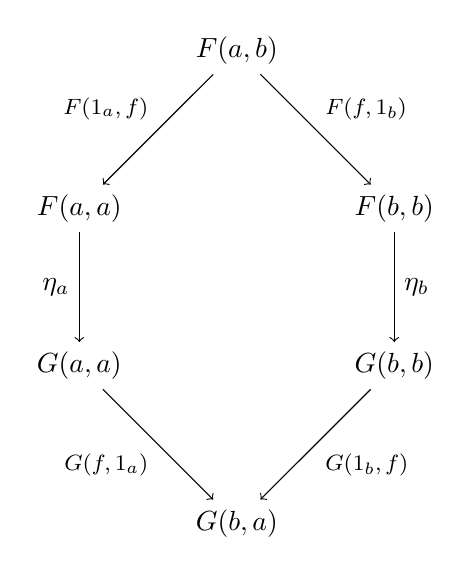
\begin{tikzpicture}
				\node (ab) at (0, 6) {$F(a, b)$};
				\node (F1) at (-2, 4) {$F(a, a)$};
				\node (F2) at (2, 4) {$F(b, b)$};
				\node (G1) at (-2, 2) {$G(a, a)$};
				\node (G2) at (2, 2) {$G(b, b)$};
				\node (ba) at (0, 0) {$G(b, a)$};
				
				\draw[->] (ab) edge node[above left]{\footnotesize$F(\mathbbm{1}_a, f)$} (F1) (F1) edge node[left]{$\eta_a$} (G1) (G1) edge node[below left]{\footnotesize$G(f, \mathbbm{1}_a)$} (ba);
				\draw[->] (ab) edge node[above right]{\footnotesize$F(f, \mathbbm{1}_b)$} (F2) (F2) edge node[right]{$\eta_b$} (G2) (G2) edge node[below right]{\footnotesize$G(\mathbbm{1}_b, f)$} (ba);
			\end{tikzpicture}
			\caption{Dinatural transformation.}
			\label{fig:dinatural}
		\end{figure}
	}

	\begin{definition}[Functor category]\index{functor!category}
		Let $C$ be a small category and let $D$ be a category. The functors $\func{F}{C}{D}$ form the objects of a category with the natural transformations as morphisms. This category is denoted by $[\textbf{C}, \textbf{D}]$ or $\textbf{D}^{\textbf{C}}$ (analogous to \ref{set:function_set}).
	\end{definition}
	
	\newdef{Representable functor}{\index{functor!representable}
		Let $\textbf{C}$ be a locally small category. A functor $\func{F}{C}{Set}$ is said to be representable if there exists an object $X\in\ob{C}$ such that $F$ is naturally isomorphic to $h^X$. The pair $(X, \psi)$, where $\psi$ is the natural isomorphism, is called a \textbf{representation} of $F$.
	}
	\remark{A similar definition exists for contravariant functors $G:\textbf{C}^{op}\rightarrow\textbf{Set}$. In this case hom$(X, -)$ has to be replaced by hom$(-, X)$.}
	
	\begin{theorem}[Yoneda's lemma]\index{Yoneda!lemma}
		Let $\textbf{C}$ be a locally small category and let $\func{F}{C}{Set}$ be a functor. For every object $X\in\ob{C}$ there exists a natural isomorphism\footnotemark\ between the set of natural transformations \emph{Nat}$(h^X, F)$ and $FX$. The image of a natural transformation $\psi\in\text{Nat}(h^X, F)$ is given by $\psi_X(\mathbbm{1}_X)$.
		\footnotetext{Here we used the fact that Nat$(h^-, -)$ can be seen as a functor $\textbf{Set}^{\textbf{C}}\times\textbf{C}\rightarrow\textbf{Set}$.}
	\end{theorem}
	\remark{For contravariant functors $G:\textbf{C}^{op}\rightarrow\textbf{Set}$ one obtains a similar statement after replacing hom$(X, -)$ by hom$(-, X)$.}

	\begin{result}[Yoneda embedding]
		When $F$ is another hom-functor $h^Y$ we obtain the following result:
		\begin{gather}
			\text{Nat}(h^X, h^Y)\cong\textbf{C}(Y, X)
		\end{gather}
		where one should pay attention to the right hand side where $Y$ appears in the first argument.
		
		Let $\text{hom}(f, -)$ denote the natural transformation corresponding to the morphism $f\in\textbf{C}(Y,X)$. The functor $h^-$ mapping an object $X\in\ob{C}$ to its hom-functor $\textbf{C}(X, -)$ and a morphism $f\in\textbf{C}(Y, X)$ to the natural transformation hom$_C(f, -)$ can also be interpreted as a covariant functor $G:\textbf{C}^{op}\rightarrow\textbf{Set}^{\textbf{C}}$. This way we see that Yoneda's lemma gives us a fully faithful functor (i.e. an embedding) $h^-$ from the opposite category $\textbf{C}^{op}$ to the functor category $\textbf{Set}^{\textbf{C}}$.
		
		As usual all of this can be done for contravariant functors. This gives us an embedding
		\begin{gather}
			h_-:\textbf{C}\hookrightarrow\textbf{Set}^{\textbf{C}^{op}}
		\end{gather}
		called the Yoneda embedding. 
	\end{result}
	
\subsection{Adjunctions}

	\newdef{Hom-set adjunction}{\index{adjunction}
		Let $\func{F}{C}{D}$ and $\func{G}{D}{C}$ be two functors. These functors form a hom-set adjunction (often just called an adjunction) if the following isomorphism is natural in $a, b$:
		\begin{gather}
			\text{hom}_D(Fa, b)\cong\text{hom}_C(a, Gb)
		\end{gather}
		The functor $F$ (resp. G) is called the left (resp. right) adjoint\footnote{Sometimes the word \textbf{adjunct} is used (French versus Latin).}.
	}
	\begin{notation}
		An adjunction$(F, G)$ between categories $\mathbf{C}, \mathbf{D}$ is often denoted by: \[\textbf{C}\adj{F}{G}\textbf{D}\] or if the ambient categories are clear by: \[F\dashv G\]
	\end{notation}
	
	\newdef{Unit-counit adjunction}{\index{triangle!identities}\index{unit}\index{zig-zag|see{triangle identity}}
		Let $\func{F}{C}{D}$ and $\func{G}{D}{C}$ be two functors. These functors form a unit-counit adjunction if there exist natural transformations
		\begin{align}
			\varepsilon: F\circ G\Rightarrow 1_D\\
			\eta: 1_C\Rightarrow G\circ F
		\end{align}
		such that the following compositions are identity morphisms:
		\begin{align}
			F\xrightarrow{F\eta}FGF\xrightarrow{\varepsilon F}F\\
			G\xrightarrow{\eta G}GFG\xrightarrow{G\varepsilon}G
		\end{align}
		These identities are sometimes called the \textbf{triangle identities} or \textbf{zig-zag identities} (the latter results from the shape of the associated string diagram). The transformations $\eta$ and $\varepsilon$ are called the \textbf{unit} and \textbf{counit} respectively.
	}
	
	\begin{property}
		Every hom-set adjuction induces a unit-counit adjunction. Let $\Phi_{a, b}$ be the natural isomorphism associated to the hom-set adjunction $F\dashv G$. The unit $\varepsilon_d$ is obtained as the adjunct $\Phi^{-1}_{Gd, d}(1_{Gd})$ of the identity morphism on $Gd\in\ob{C}$ and the counit $\eta_c$ is analogously defined as the adjunct $\Phi_{c, Fc}(1_{Fc})$ of the identity morphism at $Fc\in\ob{D}$.
		
		Similarly every unit-counit adjunction induces a hom-set adjunction. Consider a morphism $f:Fc\rightarrow d$. The (right) adjunct $\tilde{f}$ is defined as the composition \[Gf\circ\eta_c:c\rightarrow (G\circ F)c\rightarrow Gd\] Similarly, consider a morphism $\tilde{g}:c\rightarrow Gd$. The (left) adjunct $g$ is defined as the composition \[\varepsilon_d\circ F\tilde{g}: Fc\rightarrow (F\circ G)d\rightarrow d\]
	\end{property}

	Now it should be obvious that the above definition of a unit-counit adjunction can be generalized to general 2-categories:
	\newdef{Adjunction in 2-category}{\index{adjunction}
		Let \textbf{C} be a 2-category. An adjunction in \textbf{C} is a pair of 1-morphisms $F:a\rightarrow b$ and $G:b\rightarrow a$ together with 2-morphisms $\varepsilon:F\circ G\Rightarrow 1_b$ and $\eta:1_a\Rightarrow G\circ F$ that satisfy the zig-zag identities.
	}
	
	\begin{remark}[Duals and adjunctions]
		If one looks at the defining relations of duals in a rigid monoidal category one should see that these are in fact the same as the defining relations of the unit and counit of an adjunction. This is a consequence of the fact that a 2-category with a single object can be regarded as a (strict) monoidal category where the composition in the 2-category becomes the tensor product in the monoidal category. Similarly adjoint 1-morphisms in the 2-category become duals in the monoidal category.
	\end{remark}

\subsection{Constructions}

	\newdef{Discrete fibration}{\index{fibration}
		Let $\func{F}{A}{B}$ be a functor. $F$ is a discrete fibration if for every object $A\in\ob{A}$ and every morphism $f:B\rightarrow FA$ in $\textbf{B}$ there exists a unique morphism $g:C\rightarrow A$ in $\textbf{A}$ such that $F(g) = f$, where $B\in\ob{B}, C\in\ob{A}$.
	}

	\newdef{Dagger category\footnotemark}{\index{category!dagger}\index{involution}\label{cat:dagger_category}
		\footnotetext{Also called a \textbf{$\dag$-category}.}
		A category equipped with a contravariant endofunctor, i.e. a functor $\dag:\textbf{C}^{op}\rightarrow\textbf{C}$, such that:
		\begin{enumerate}
			\item $\forall C\in\ob{C}: \mathbbm{1}_C^\dag = \mathbbm{1}_C$
			\item $\dag\circ\dag = \mathbbm{1}_C$
		\end{enumerate}
		The second property says that $\dag$ is an \textbf{involutive} functor.
	}
	\remark{The concept of a dagger structure allows the usual definition of \textbf{unitary} and \textbf{self-adjoint} morphisms.}\index{unitary}
	\begin{property}
		The unitary morphisms in a dagger category form a groupoid\footnote{See definition \ref{cat:groupoid}.}.
	\end{property}
	
	\newdef{Comma category}{\index{category!comma}
		Let $\textbf{A}, \textbf{B}$ and $\textbf{C}$ be three categories and let $\func{F}{A}{C}$ and $\func{G}{B}{C}$ be two functors. The comma category $F\downarrow G$ is defined as follows:
		\begin{itemize}
			\item Objects are triples $(A, B, \gamma)$ where $A\in\ob{A}, B\in\ob{B}$ and $\gamma:FA\rightarrow GB\in\text{hom}(\textbf{C})$.
			\item Morphisms $(A, B, \gamma)\rightarrow(K, L, \sigma)$ are pairs $(f, g)$ where $f:A\rightarrow K\in\text{hom}(\textbf{A})$ and $g:B\rightarrow L\in\text{hom}(\textbf{B})$ such that $\sigma\circ F(f) = G(g)\circ\gamma$.
			\item Composition of morphisms is defined componentwise.
		\end{itemize}
	}
	\newdef{Slice category}{\index{category!slice}
		Let \textbf{C} be a category and let $c\in\ob{C}$. The slice category $\textbf{C}/c$ of $\textbf{C}$ over $c$ is defined as follows:
		\begin{itemize}
			\item The objects are morphisms in $\textbf{C}$ with codomain $c$.
			\item The morphisms $f\rightarrow g$ are morphisms $h$ in $\textbf{C}$ such that $g\circ h = f$.
		\end{itemize}
	}
	
\subsection{Monads}

	\newdef{Monad}{\index{monad}
		A monad is a triple $(T, \mu, \eta)$ where $\func{T}{C}{C}$ is an endofunctor and $\mu:T^2\rightarrow T, \eta:\text{id}_{\mathbf{C}}\rightarrow T$ are natural transformations satisfying the following (coherence) conditions:
		\begin{enumerate}
			\item As natural transformation from $T^3$ to $T$ we have:
			\begin{gather}
				\mu\circ T\mu = \mu\circ\mu_T
			\end{gather}
			\item As natural transformation from $T$ to itself we have:
			\begin{gather}
				\mu\circ T\eta = \mu\circ\eta_T = \mathbbm{1}
			\end{gather}
		\end{enumerate}
		These conditions say that a monad is a monoid in the category $\mathbf{End}_{\mathbf{C}}$ of endofunctors on $\mathbf{C}$.
	}
	\begin{example}[Adjunction]
		Every adjunction $F\dashv G$, with unit $\varepsilon$ and counit $\eta$, induces a monad of the form $(GF, G\varepsilon F, \eta)$.
	\end{example}
	
	\newdef{Algebra\footnotemark\ over a monad}{\index{algebra!over a monad}
		\footnotetext{A more suitable name would be ''module over a monad'', since these are modules over a monoid if we view monads as monoids in $\mathbf{End}_{\mathbf{C}}$.}
		Consider a monad $(T, \mu, \eta)$ on a category $\mathbf{C}$. A algebra over $T$ is a couple $(a, \kappa)$ where $a\in\ob{C}$ and $\kappa:Ta\rightarrow a$ such that the following conditions are satisfied:
		\begin{enumerate}
			\item $\kappa\circ T\kappa = \kappa\circ\mu_a$
			\item $\kappa\circ\eta_a = \mathbbm{1}_a$
		\end{enumerate}
		Morphisms $(a, \kappa_a)\rightarrow(b, \kappa_b)$ of $T$-algebras are morphisms $f:a\rightarrow b$ in $\mathbf{C}$ such that $f\circ\kappa_a = \kappa_b\circ Tf$.
	}
	\newdef{Eilenberg-Moore category}{\index{Eilenberg-Moore}
		Given a monad $T$ over a category $\mathbf{C}$ we define the Eilenberg-Moore category $\mathbf{C}^T$ as the category of $T$-algebras.
	}
	
	\newdef{Monadic adjunction}{
		An adjunction between categories $\mathbf{C}$ and $\mathbf{D}$ is said to be monadic if there exists an equivalence between $D$ and the Eilenberg-Moore category of the induced monad.
	}
	\newdef{Monadic functor}{\index{functor!monadic}
		A functor is said to be monadic if it admits a left adjoint such that the adjunction is monadic.
	}
	
	\begin{theorem}[Beck's monadicity theorem]
		Consider a functor $\func{F}{C}{D}$. This functor is monadic if and only if the following conditions are satisfied:
		\begin{itemize}
			\item $F$ admits a left adjoint.
			\item $F$ reflects isomorphisms.
			\item $\mathbf{C}$ has all coequalizers of $F$-split parallel pairs\footnote{These are parallel pairs $f,g$ such that the images $Ff, Fg$ under $F$ admit a split coequalizer (see definition \ref{cat:split_coequalizer}).} and $F$ preserves these coequalizers.
		\end{itemize}
	\end{theorem}
	\remark{A sufficient condition for monadicity is obtained by replacing the third item above by the following weaker statement: ''$\mathbf{C}$ has all coequalizers of reflexive pairs and $F$ preserves these coequalizers.'' This weaker form is called the \textbf{crude monadicity theorem}.}

	\newdef{Closure operator\footnotemark}{\label{cat:closure_operator}\index{closure!operator}\index{modal operator|see{closure operator}}
		\footnotetext{Also called a \textbf{modal operator}.}
		Consider a monad $\func{T}{C}{C}$ with unit and product maps $\eta, \mu$. This monad is called a closure operator if the product map is a natural isomorphism.
		
		Given a closure operator $\func{T}{C}{C}$, one calls the object $Tx$ the closure of $x\in\ob{C}$. The \textbf{closing map} of an object $x\in\ob{C}$ is defined as the morphism $\eta_x$ and $x$ is said to be $T$\textbf{-closed} exactly if its closing map is an isomorphism.
	}

\section{Initial and terminal objects}

	\newdef{Initial object}{
		An object $O$ in a category $\textbf{C}$ is called initial if for every other object $P$ there exists a unique morphism $\iota_P:O\rightarrow P$.
	}
	\newdef{Terminal object}{
		An object $O$ in a category $\textbf{C}$ is called terminal if for every other object $P$ there exists a unique morphism $\tau_P:P\rightarrow O$. This object is sometimes denoted by $\mathbf{1}$.
	}
	\begin{property}
		If an initial (resp. terminal) object exists, then it is unique (possibly up to isomorphism).
	\end{property}
	\newdef{Well-pointed category}{
		A category is said to be well-pointed if the terminal object is a generator\footnote{See definition \ref{cat:generator}.}.
	}
	
	\newdef{Zero object}{\index{zero!object}\label{cat:zero_object}
		An object which is both initial and terminal. The zero object is often denoted by $\mathbf{0}$.
	}
	\begin{property}[Zero morphism]
		From the definition of the zero object it follows that for any two objects $A, B$ there exists a unique morphism $0_{AB}:A\rightarrow0\rightarrow B$.
	\end{property}
	\newdef{Pointed category}{\index{pointed!category}
		A category is said to be pointed if it contains a zero object.
	}
	
	\newdef{Global element}{\index{global!element}\label{category:global_element}
		Let $\textbf{C}$ be a category with terminal object $\mathbf{1}$. A global element of an object $X\in\ob{C}$ is a morphism $\mathbf{1}\rightarrow X$.
	}
	\newdef{Pointed object}{\index{pointed!object}
		An object $X$ equipped with a global element $1\rightarrow X$ (which is sometimes called the \textbf{basepoint}).
	}
	
	\begin{remark}
		In the category \textbf{Set} the elements of a set $S$ are in one-to-one correspondence with the global elements of $S$ and one has the important property (axiom) that two functions $f, g:S\rightarrow S'$ coincide if their evaluation at every element $s\in S$ is equal or equivalently if the precompositions with global elements coincide.
		
		However this way of checking equality can fail in other categories. Consider for example \textbf{Grp}. In this category the terminal object is $0 = \{e\}$. The only morphism from this group to any other group $G$ is the one mapping $e$ to the unit in $G$ ($0$ is also an initial object in \textbf{Grp}). It is obvious that precomposition with this morphism tells us nothing about the equality of other morphisms. To recover the technique used in \textbf{Set} one needs to generalize the notion of "element":
	\end{remark}
	\newdef{Generalized element}{\index{shape}
		Let $\textbf{C}$ be category and consider an object $X$ in $\textbf{C}$. For any object $Y\in\ob{C}$ one calls a morphism $Y\rightarrow X$ a generalized element of $X$. The morphisms $Y\rightarrow X$ are also called $\textbf{Y-elements}$ in $X$ or elements of \textbf{shape} $Y$ in $X$.
	}

\section{Diagrams and universal constructions}

	\newdef{Diagram}{\index{diagram}
		A diagram in $\textbf{C}$ with index category $\textbf{I}$ is a (covariant) functor $\func{D}{I}{C}$.
	}
	
	\newdef{Cone}{\index{cone}
		Let $\func{D}{I}{C}$ be a diagram. A cone from $a\in\ob{C}$ to $D$ consists of a family of morphisms $\psi_i:a\rightarrow Di, \forall i\in\ob{I}$ such that $\psi_j = Df\circ\psi_i$ for all morphisms $f:i\rightarrow j\in\text{hom}(\textbf{I})$, as depicted in figure \ref{fig:cone_component}.
		
		\begin{figure}[ht!]
			\centering
			\begin{subfigure}[b]{0.49\textwidth}
				\centering
				\begin{tikzpicture}
					\matrix (m) [matrix of math nodes,row sep=3em,column sep=3em, minimum width=1em, ampersand replacement=\&]{
						\&a\&\\
						Di\vphantom{(}\&\&Df(i)\\
					};
					\draw[->] (m-1-2) -- (m-2-1) node[pos=0.5, above left]{$\psi_i$};
					\draw[->] (m-1-2) -- (m-2-3) node[pos=0.5, above right]{$\psi_{f(i)}$};
					\draw[->] (m-2-1) -- (m-2-3) node[pos=0.5, below]{$Df$};
				\end{tikzpicture}
				\caption{Component of cone over $D$.}
				\label{fig:cone_component}
			\end{subfigure}
			\begin{subfigure}[b]{0.49\textwidth}
				\centering
				\begin{tikzpicture}
					\matrix (m) [matrix of math nodes,row sep=3em,column sep=3em, minimum width=1em, ampersand replacement=\&]{
						a\vphantom{b}\&\&b\\
						\&Di\&\\
					};
					\draw[->] (m-1-1) -- (m-2-2) node[pos=0.5, below left]{$\psi_i$};
					\draw[->] (m-1-3) -- (m-2-2) node[pos=0.5, below right]{$\phi_i$};
					\draw[->] (m-1-1) -- (m-1-3) node[pos=0.5, above]{$f$};
				\end{tikzpicture}
				\caption{Morphism of cones.}
				\label{fig:cone_morphism}
			\end{subfigure}
			\label{fig:cone}
		\end{figure}
	}
	\begin{adefinition}\index{diagonal!functor}
		This definition can be reformulated by defining an additional functor\footnote{The notation $\Delta_a$ tells us that $\Delta:C\rightarrow [\textbf{I},\textbf{C}]$ is the \textbf{diagonal functor}, i.e. $\Delta_c\equiv\Delta(c)$ is the constant functor from $\textbf{I}$ to $\textbf{C}$ with target object $c$.} $\Delta_a:\textbf{I}\rightarrow\textbf{C}$ which maps every element $i\in\ob{I}$ to $a$ and every morphism $g\in\text{hom}(\textbf{I})$ to id$_a$. The morphisms $\psi_c$ can then be seen as the components of a natural transformation $\psi:\Delta_a\Rightarrow D$. Hence a cone $(a, \psi)$ is an element of $[\textbf{I}, \textbf{C}](\Delta_a, D)$.
	\end{adefinition}

	\newdef{Morphism of cones}{\index{morphism!of cones}
		Let $\func{D}{I}{C}$ be a diagram and let $(a, \psi), (b, \phi)$ be cones to $D$. A morphism between these cones is a morphism of the apexes $f:a\rightarrow b$ such that the diagrams of the form \ref{fig:cone_morphism} commute for all $i\in\ob{I}$. The cones to $D$ together with these morphisms form a category $\textbf{Cone}(D)$, in fact this can easily be seen to be the comma category $(\Delta \downarrow D)$.
	}
	
	\newdef{Limit}{\index{limit}
		Consider a diagram $\func{D}{I}{C}$. The limit $\lim D$ of this diagram, if it exists, is the terminal object of the category $\textbf{Cone}(D)$.
	}
	This definition gives us the following universal property:
	\begin{uproperty}
		Let $\func{D}{I}{C}$ be a diagram and let $\lim D$ be its limit. For every cone $(a, \psi)\in\textbf{Cone}(D)$ there exists a unique morphism $f:c\rightarrow\lim D$.
	\end{uproperty}
	
	\begin{example}[Terminal object]
		A terminal object $\mathbf{1}$ is a limit over the empty diagram.
	\end{example}
	
	\newdef{Continuous functor}{\index{continuity!functor}\label{cat:continuity}
		A functor which preserves all small limits.
	}
	\begin{property}
		In a locally small category every hom-functor is continuous\footnote{They even preserve limits which are not necessarily small.}.
	\end{property}
	
	\newdef{Equalizer}{\index{equalizer}\index{fork}
		Consider the following diagram:\[X\overset{f}{\underset{g}{\rightrightarrows}} Y\] The limit of this diagram is called the equalizer of $f$ and $g$. Explicitly the equalizer is the universal object $E$ together with a morphism $e: E\rightarrow X$ such that $f\circ e = g\circ e$. By dualization one obtains a cofork
	}
	\newdef{Split coequalizer}{\label{cat:split_coequalizer}
		First we define a \textbf{cofork} diagram, i.e. a diagram \[a\overset{f}{\underset{g}{\rightrightarrows}} b\overset{t}{\rightarrow} c\] where $t\circ f = t\circ g$. A split coequalizer\footnote{A coequalizer, as obtained by dualizing the previous definition, is just a universal cofork.} is a cofork together with a section $\varphi$ of $f$ and a section $\sigma$ of $t$ such that $\sigma\circ t = g\circ \varphi$.
	}
	
	\newdef{Finitely complete category}{\index{finitely!complete}
		A category is said to be finitely complete if it has a terminal object and if all binary equalizers and products exist.
	}
	\newadef{Finitely complete category}{
		A category is said to be finitely complete if all finite limits exist.
	}
	
	\newdef{Span}{\index{span}
		A span in a category $C$ is a diagram of the form \ref{fig:cat_span}.
		
		Let $\Lambda$ be the category with three objects $\{-1, 0, 1\}$ and two morphisms $i:0\rightarrow -1$ and $j:0\rightarrow 1$. By the above definition of a diagram a span in $C$ is equivalent to a functor $\func{S}{\Lambda}{C}$.
	}
	
	\newdef{Pullback\footnotemark}{\index{pullback}\label{cat:pullback}
		\footnotetext{Also called a \textbf{fibre product} or \textbf{Cartesian square}.}
		The pullback of two morphisms $f:A\rightarrow C$ and $g:B\rightarrow C$ is defined as the limit of cospan \ref{fig:pullback}.
	}
	\begin{figure}[!ht]
		\centering
		\begin{subfigure}[b]{0.49\textwidth}
			\centering
			\begin{tikzpicture}
				\matrix (m) [matrix of math nodes,row sep=2em,column sep=2em, minimum width=1em, ampersand replacement=\&]{
					\&S\&\\
					A\&\&B\\
				};
				\draw[->] (m-1-2) -- (m-2-1) node[pos=0.5, above left]{$f$};
				\draw[->] (m-1-2) -- (m-2-3) node[pos=0.5, above right]{$g$};
			\end{tikzpicture}
			\caption{Span (category theory).}
			\label{fig:cat_span}
		\end{subfigure}
		\begin{subfigure}[b]{0.49\textwidth}
			\centering
			\begin{tikzpicture}
				\matrix (m) [matrix of math nodes,row sep=2em,column sep=2em, minimum width=1em, ampersand replacement=\&]{
					A\&\&B\\
					\&C\&\\
				};
				\draw[->] (m-1-1) -- (m-2-2) node[pos=0.5, below left]{$f$};
				\draw[->] (m-1-3) -- (m-2-2) node[pos=0.5, below right]{$g$};
			\end{tikzpicture}
			\caption{Cospan.}
			\label{fig:pullback}
		\end{subfigure}
		\caption{}
	\end{figure}
	
	\begin{notation}[Pullback]
		The pullback of two morphisms $f:A\rightarrow C$ and $g:B\rightarrow C$ is often denoted by $A\times_C B$.
	\end{notation}
	
	\begin{property}
		If a terminal object $\mathbf{1}$ exists then the pullback $A\times_{\mathbf{1}}B$ is equal to the (Cartesian) product  $A\times B$.
	\end{property}
	\newdef{Pushout}{\index{pushout}
		The dual notion of a pullback, i.e. the colimit of a span.
	}

	\newdef{Wedge}{\index{wedge}
		Consider a profunctor $F:\mathbf{C}^{op}\times\mathbf{C}\rightarrow\mathbf{Set}$. A wedge $e:w\rightarrow F$ is an object $w\in\ob{Set}$ together with a collection of morphisms $e_c:w\rightarrow F(c, c)$ indexed by $\ob{C}$ such that for any morphism $f:c\rightarrow c'$ the following diagram commutes:
		\begin{gather*}
			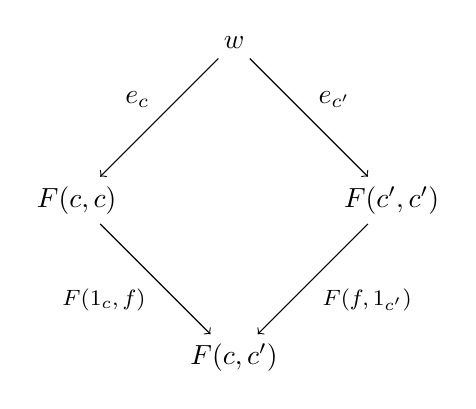
\begin{tikzpicture}
				\node (W) at (0, 4) {$w$};
				\node (F1) at (-2, 2) {$F(c, c)$};
				\node (F2) at (2, 2) {$F(c', c')$};
				\node (F) at (0, 0) {$F(c, c')$};
				\draw[->] (W) edge node[above left]{$e_c$} (F1) (F1) edge node[below left]{\footnotesize$F(\mathbbm{1}_c, f)$} (F);
				\draw[->] (W) edge node[above right]{$e_{c'}$} (F2) (F2) edge node[below right]{\footnotesize$F(f, \mathbbm{1}_{c'})$} (F);
			\end{tikzpicture}
		\end{gather*}
		As was the case for cones, one can reformulate this in terms of (di)natural transformations. A wedge $(w, e)$ of a profunctor $F:\mathbf{C}^{op}\times\mathbf{C}\rightarrow\mathbf{Set}$ is a dinatural transformation from the constant profunctor $\Delta_w$ to $F$.
	}
	\newdef{End}{\index{end}
		The end of a profunctor $F:\mathbf{C}^{op}\times\mathbf{C}\rightarrow\mathbf{Set}$ is defined as the universal wedge of $F$. The components of the wedge are called the \textbf{projection maps} of the end. This stems from the fact that for a discrete category the end coincides with the product $\prod_{c\in\ob{C}}F(c, c)$.
	}
	\newnot{End}{
		The end of a profunctor $F:\mathbf{C}^{op}\times\mathbf{C}\rightarrow\mathbf{Set}$ is often denoted using an integral sign with subscript: \[\int_{c\in\mathbf{C}}F(c, c)\] For the dual construction, i.e. a \textbf{coend}, one uses the integral sign with superscript.
	}
	\begin{example}[Natural transformations]
		Consider two functors $\func{F, G}{C}{D}$. The map $(c, c')\mapsto\mathbf{D}(Fc, Gc')$ gives a profunctor $H:\mathbf{C}^{op}\times\mathbf{C}\rightarrow\mathbf{Set}$. If we look at the wedge condition for this profunctor (especially the lower half) we get the following equality for all morphisms $f:c\rightarrow c'$:
		\begin{gather}
			\tau_{c'}\circ Ff = Gf\circ \tau_c
		\end{gather}
		where $\tau_c$ is the projection of the wedge associated to the object $c\in\ob{C}$. Comparing this equality to definition \ref{cat:natural} we immediately see that the end $\int_{c\in\mathbf{C}}\mathbf{D}(Fc, Gc)$ is exactly Nat$(F, G)$.
	\end{example}
	
	\begin{property}
		Using the continuity\footnote{See definition \ref{cat:continuity}.} of the hom-functor one can prove the following equality which can be used to turn ends into coends and vice versa:
		\begin{gather}
			\mathbf{Set}\left(\int^{c\in\mathbf{C}}F(c, c), c'\right) = \int_{c\in\mathbf{C}}\mathbf{Set}\left(F(c, c), c'\right)
		\end{gather}
	\end{property}
	
	Using the above properties and definitions one obtains the following Yoneda-like statements:
	\begin{theorem}[Ninja Yoneda lemma]\index{Yoneda!lemma}
		Let $\func{F}{C}{D}$ be a covariant functor. The following two isomorphisms follow from the ordinary Yoneda lemma (and the above property):
		\begin{gather}
			\int_{c'\in\mathbf{C}}\mathbf{Set}\left(\mathbf{C}(c, c'), Fc'\right)\cong Fc
		\end{gather}
		\begin{gather}
			\int^{c\in\mathbf{C}}\mathbf{C}(c, c')\times Fc\cong Fc'
		\end{gather}
	\end{theorem}
	
	\newdef{Kan extension}{\index{Kan!extension}
		Consider two functors $\func{F}{C}{D}$ and $\func{G}{C}{E}$. The right Kan extension\footnote{The left Kan extension Lan$_GF$ is obtained by dualizing this construction (flipping the direction of the natural transformation).} of $F$ along $G$ is given by the universal functor $\func{\text{Ran}_GF}{E}{D}$ and natural transformation $\eta:\text{Ran}_GF\circ G\Rightarrow F$:
		\begin{gather*}
			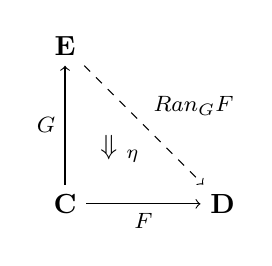
\begin{tikzpicture}
				\node (E) at (0, 2) {$\mathbf{E}$};
				\node (C) at (0, 0) {$\mathbf{C}$};
				\node (D) at (2, 0) {$\mathbf{D}$};
				\node (A) at (0.7, 0.7) {$\Downarrow_{\ \eta}$};
				\draw[->] (C) -- node[left]{\footnotesize$G$} (E);
				\draw[->] (C) -- node[below]{\footnotesize$F$} (D);
				\draw[dashed, ->] (E) -- node[above right]{\footnotesize$\text{Ran}_GF$} (D);
			\end{tikzpicture}
		\end{gather*}
		Universality means that every other natural transformation $\chi:H\circ G\Rightarrow F$ factors uniquely through $\eta$.
	}
	\begin{example}[Limit]
		Denote the terminal category by $\mathbf{1}$. By choosing the functor $G$ in the definition of a right Kan extension to be the unique functor $!_C:\mathbf{C}\rightarrow\mathbf{1}$ into the terminal category one obtains the definition of a limit, i.e. $\lim F = \text{Ran}_{!_C}F$. Similarly one can obtain the colimit as the left Kan extension.
	\end{example}
	
	\newdef{Absolute Kan extension}{
		A (left) Kan extension Lan$_GF$ is said to be absolute if for every functor $H$ with the same codomain as $F$ the following isomorphism holds:
		\begin{gather}
			H(\text{Lan}_GF)\cong\text{Lan}_G(HF)
		\end{gather}
		There exists an analogous definition for right Kan extensions.
	}

	\newadef{Kan extension}{
		The construction above gives a functor Ran$_G$ from the functor category $[\mathbf{C}, \mathbf{D}]$ to the functor category $[\mathbf{E}, \mathbf{D}]$. The right Kan extension Ran$_G$ can be defined as the right adjoint to the pullback functor $G^*:F\mapsto F\circ G$. Similarly one can define the left Kan extension as the left adjoint to the pullback functor $G^*$.
	}
	\remark{Using this equivalence of hom-spaces one can generalize the Kan extension from $\mathbf{Cat}$ to any 2-category.}
	
	The existence of Kan extensions can also be used to determine the existence of adjoints:
	\begin{property}
		A functor $\func{F}{C}{D}$ admits a left adjoint\footnote{An analogous statement holds for right adjoints.} if and only if the right Kan extension of the identity functor $\func{\mathbbm{1}}{C}{C}$ along $F$ exists. If it exists and if it is an absolute extension then the left adjoint is given exactly by this Kan extension.
	\end{property}
	
\section{Morphisms}

	\newdef{Section}{\index{section}
		A section of a morphism $f:a\rightarrow b$ is a right-inverse, i.e. a morphism $g:b\rightarrow a$ such that $f\circ g=\mathbbm{1}_b$.
	}
	\newdef{Monomorphism}{\index{monomorphism}
		Let \textbf{C} be a category. A morphism $\mu\in\textbf{C}(A, B)$ is called a mono\footnote{Sometimes just a \textbf{mono} or a \textbf{monic} morphism.} if for every object $X\in\ob{C}$ and every two morphisms $\alpha_1, \alpha_2\in\textbf{C}(X, A)$ such that $\mu\circ\alpha_1 = \mu\circ\alpha_2$ we can conclude that $\alpha_1=\alpha_2$.
	}
	\newdef{Epimorphism}{\index{epimorphism}
		Let \textbf{C} be a category. A morphism $\varepsilon\in\textbf{C}(A, B)$ is called an epimorphism\footnote{Sometimes just an \textbf{epi} or an \textbf{epic} morphism.} if for every object $X\in\ob{C}$ and every two morphisms $\alpha_1, \alpha_2\in\textbf{C}(B, X)$ such that $\alpha_1\circ\varepsilon = \alpha_2\circ\varepsilon$ we can conclude that $\alpha_1=\alpha_2$.
	}
	
	\newdef{Balanced category}{\index{category!balanced}\label{category:balanced}
		A category is said to be balanced if every monic epi is an isomorphism.
	}
	
	\begin{property}[Global elements]
		Every global element\footnote{See definition \ref{category:global_element}.} is monic.
	\end{property}
	
	\newdef{Reflexive pair}{
		Two parallel morphisms $f, g:a\rightarrow b$ are said to form a reflexive pair if they have a common section, i.e. there exists a morphism $\sigma:b\rightarrow a$ such that $f\circ\sigma=g\circ\sigma$.
	}
	
	\begin{property}[Equalizing morphism]
		Consider an equalizer $(E, e)$. The equalizing morphism $e$ is monic. Similarly a coequalizing morphism is epic.
	\end{property}

	\newdef{Regular monomorphism}{\index{regular!morphism}
		A mono is said to be regular if it arises as an equalizer of two parallel morphisms.
	}
	\begin{property}[Regular bimorphism]\label{category:regular_iso}
		A monic regular epimorphism is an isomorphism. Analogously so is an epic regular monomorphism is an isomorphism.
	\end{property}
	
	\newdef{Injective object}{\index{injective!object}
		Let \textbf{C} be an category. An object $I\in\ob{C}$ is said to be injective if for every $A, B\in\ob{C}$, mono $f:A\rightarrow B$ and morphism $g:A\rightarrow I$ there exists a morphism $\phi:B\rightarrow I$ such that $\phi\circ f = g$.
		\begin{figure}[ht!]
			\centering
			\begin{subfigure}[b]{0.49\textwidth}
				\centering
				\begin{tikzpicture}
					\matrix (m) [matrix of math nodes,row sep=7em,column sep=7em, minimum width=2em, ampersand replacement=\&]{
						A\&B\\
						I\&\\
					};
					\draw[right hook ->] (m-1-1) -- (m-1-2) node[pos=0.5, above]{$f$};
					\draw[->] (m-1-1) -- (m-2-1) node[pos=0.5, left]{$g$};
					\draw[dashed, ->] (m-1-2) -- (m-2-1) node[pos=0.5, below right]{$\phi$};
				\end{tikzpicture}
				\caption{Injective object $I$.}
				\label{fig:injective_object}
			\end{subfigure}
			\begin{subfigure}[b]{0.49\textwidth}
				\centering
				\begin{tikzpicture}
					\matrix (m) [matrix of math nodes,row sep=7em,column sep=7em, minimum width=2em, ampersand replacement=\&]{
						A\&B\\
						\&P\\
					};
					\draw[->>] (m-1-1) -- (m-1-2) node[pos=0.5, above]{$f$};
					\draw[->] (m-2-2) -- (m-1-2) node[pos=0.5, right]{$g$};
					\draw[dashed, ->] (m-2-2) -- (m-1-1) node[pos=0.5, below left]{$\phi$};
				\end{tikzpicture}
				\caption{Projective object $P$.}
				\label{fig:projective_object}
			\end{subfigure}
		\end{figure}
	}
	
	Dually one can construct:
	\newdef{Projective object}{\index{projective!object}
		Let \textbf{C} be an category. An object $P\in\ob{C}$ is said to be projective if for every $A, B\in\ob{C}$, epi $f:A\rightarrow B$ and morphism $g:P\rightarrow A$ there exists a morphism $\phi:P\rightarrow B$ such that $f\circ\phi = g$.
	}
	
	\newdef{Subobject}{\index{subobject}
		Let \textbf{C} be a category and let $A\in\ob{C}$ be any object. A subobject $B$ of $A$ is a mono $B\hookrightarrow A$.
		
		In fact one should work up to isomorphism and hence the complete definition goes as follows. A subobject $B$ of $A$ in the category \textbf{C} is an isomorphism class of monos $i:B\hookrightarrow A$ in the slice category $\textbf{C}/A$.
	}
	\newdef{Well-powered category}{\index{category!well-powered}
		A category \textbf{C} is said to be well-powered if for every object $A\in\ob{C}$ the class of subobjects \textbf{Sub}$(A)$ is small.
	}
	
	\newdef{Generator\footnotemark}{\index{generator}\label{cat:generator}
		\footnotetext{Also called a \textbf{separator}.}
		Let \textbf{C} be a category. A collection of objects $\{O_i\in\ob{C}\}$ is called a collection of generators for \textbf{C} if, given any two objects $A, B\in\ob{C}$ and any two morphisms $f, g:A\rightarrow B$, we have that $f\neq g\implies\exists j\in I, h_j\in\textbf{C}(O_i, A): f\circ h_j\neq g\circ h_j$.
	}
	
	\newdef{Decategorification}{
		Let \textbf{C} be a (essentially) small category. The set of isomorphism classes of \textbf{C} is called the decategorification of \textbf{C}. This is given by a functor \[K:\textbf{Cat}\rightarrow\textbf{Set}\]
	}
	
	\newdef{Lift}{\index{lift}
		A lift of a morphism $f:A\rightarrow B$ along an epi $e:X\rightarrow B$ is a morphisms $\tilde{f}:A\rightarrow X$ satisfying $f = e\circ\tilde{f}$.
	}
	\newdef{Lifting property}{\index{orthogonal}
		A morphism $f:A\rightarrow B$ has the left lifting property with respect to a morphism $g:C\rightarrow D$ if for every commutative diagram
		\begin{figure}[ht!]
			\centering
			\begin{tikzcd}[ampersand replacement=\&, row sep=4em,column sep=4em, minimum width=2em]
				A \arrow[r] \arrow[d, "f"'] \& C \arrow[d, "g"]\\
				B \arrow[ur, "\psi"] \arrow[r] \& D
			\end{tikzcd}
			\caption{Left lifting property.}
			\label{fig:lifting_property}
		\end{figure}
		there exists a morphism $\psi:B\rightarrow C$ such that the triangles commute. The morphism $g$ is also said to have the right lifting property with respect to $f$. If the morphism $\psi$ is unique then $f$ and $g$ are said to be \textbf{orthogonal}.
	}
	
	\newdef{Weak factorization system}{\index{weak!factorization}\label{category:wfc}
		Consider a category \textbf{C}. A pair $(L, R)$ of classes of morphisms in \textbf{C} is called a weak factorization system (WFS) if it satisfies the folllowing 3 properties:
		\begin{enumerate}
			\item Every morphism in \textbf{C} factors as a composition $g\circ f$ where $f\in L$ and $g\in R$.
			\item $L$ consists of the morphisms in \textbf{C} that have the left lifting property with respect to morphisms in $R$.
			\item $R$ consists of the morphisms in \textbf{C} that have the right lifting property with respect to morphisms in $L$.
		\end{enumerate}
	}
	
	\newdef{Localization}{\index{localization}\label{cat:localization}
		Consider a category \textbf{C} with a collection of morphism $M\subset\text{mor}(\textbf{C})$. The localization of \textbf{C} with respect to $M$ is constructed by adding for each morphism $f\in M$ a formal inverse to $\text{mor}(\textbf{C})$.
	}

\section{Abelian categories}

	\newdef{Pre-additive category}{
		A (locally small) category enriched over \textbf{Ab}, i.e. every hom-set is an Abelian group and composition is bilinear.
	}
	\newdef{$k$-linear category}{\index{category!linear}
		Let \textbf{Vect}$_k$ denote the category of vector spaces over the base field $k$. A $k$-linear category is a category enriched over \textbf{Vect}$_k$.
	}
	
	\begin{property}\index{zero!object}
		Let \textbf{A} be a pre-additive category and let $X\in\ob{A}$. The following statements are equivalent:
		\begin{itemize}
			\item $X$ is an initial object.
			\item $X$ is a final object.
			\item $\mathbbm{1}_X$ = 0
		\end{itemize}
		Any initial/terminal object is hence a zero object\footnote{See definition \ref{cat:zero_object}.}.
	\end{property}
	\begin{property}\index{biproduct}
		In a pre-additive category the finite products $\prod_{i\in I}X_i$ are isomorphic to the finite coproducts $\bigsqcup_{i\in I} X_i$ (which are called \textbf{direct sums} in this context). If a product $X\times Y$ exists then so does the coproduct $X\sqcup Y$ and if the coproduct exists then so does the product. In general if a product and coproduct exist and are equal then one speaks of a \textbf{biproduct}.
	\end{property}
	
	\newdef{Additive category}{\index{additive!category}
		A pre-additive category in which all finite biproducts exist.
	}
	
	If one speaks of additive categories, one generally assumes that the associated functors are of a specific type:
	\newdef{Additive functor}{\index{additive!functor}\label{additive_functor}
		Let $\mathbf{A}, \mathbf{A'}$ be additive categories. A functor $\func{F}{A}{A'}$ is said to be additive if it preserves all biproducts, i.e. if it satisfies the following conditions:
		\begin{itemize}
			\item It preserves zero objects: $F0_A \cong 0_{A'}$.
			\item There exists a natural isomorphism $F(X\oplus Y)\cong FX\oplus FY$.
		\end{itemize}
		
		One can generalize this notion to pre-additive categories. A functor between pre-additive categories is said to be additive if it acts as a group morphism on hom-spaces.
	}
	
	In a pre-additive category one can define the classical notions from (homological) algebra such as images and kernels:
	\newdef{Kernel}{\index{kernel}
		Let $f:X\rightarrow Y$ be a morphism. A\footnote{Note the word \textit{a}. The kernel of a morphism is determined up to an isomoprhism.} kernel is a morphism $k:Z\rightarrow X$ such that:
		\begin{itemize}
			\item $f\circ k = 0$
			\item Universal property: for every other morphism $k':Z'\rightarrow X$ such that $f\circ k' = 0$ there exists a unique morphism $h:Z'\rightarrow Z$ such that $k\circ h = k'$.
		\end{itemize}
		Hence a kernel of $f$ is an equalizer of $f$ and 0.
	}
	\begin{notation}[Kernel]
		If the kernel of $f:X\rightarrow Y$ exists then it is denoted by $\ker(f)\rightarrow X$.
	\end{notation}
	
	\newdef{Cokernel}{
		Let $f:X\rightarrow Y$ be a morphism. A cokernel is a morphism $p:Y\rightarrow Z$ such that:
		\begin{itemize}
			\item $p\circ f = 0$
			\item Universal property: for every other morphism $p':Y\rightarrow Z'$ such that $p'\circ f = 0$ there exists a unique morphism $h:Z\rightarrow Z'$ such that $h\circ p = p'$.
		\end{itemize}
		Hence a cokernel of $f$ is a coequalizer of $f$ and 0.
	}
	\begin{notation}[Cokernel]
		If the cokernel of $f:X\rightarrow Y$ exists then it is denoted by $Y\rightarrow\text{coker}(f)$.
	\end{notation}
	\remark{The name and notation of the kernel\footnote{Similarly for the cokernel.} (in the categorical sense) is explained by remarking that by Yoneda's lemma the morphism \[\ker(f)\rightarrow X\] represents the functor \[F:Z\mapsto\ker\Big(\textbf{C}(Z, X)\rightarrow\textbf{C}(Z, Y)\Big)\]}

	\newdef{Pre-Abelian category}{
		An additive category is pre-Abelian if every morphism has a kernel and cokernel.
	}
	\newdef{Abelian category}{\index{Abelian!category}
		A pre-Abelian category in which every mono is a kernel and every epi is a cokernel or equivalently if for every morphism $f$ there exists an isomorphism $\text{coker}(\ker(f))\cong\ker(\text{coker}(f))$.
	}
	
	\begin{property}
		In Abelian categories a morphism is monic if and only if it is injective, i.e. its kernel is 0. Analogously a morphism is epic if and only if it is surjective, i.e. its cokernel is 0.
	\end{property}

	\newdef{Exact functor}{\index{exact!functor}
		Let $\func{F}{A}{A'}$ be an additive functor between additive categories. We use the following definitions:
		\begin{itemize}
			\item $F$ is said to be left exact if it preserves kernels.
			\item $F$ is said to be right exact if it preserves cokernels.
			\item $F$ is said to be exact if it is both left and right exact.
		\end{itemize}
	}
	\begin{result}
		The previous definition implies the following properties (which can in fact be used as an alternative definition):
		\begin{itemize}
			\item If $F$ is left exact it maps an exact sequence of the form \[0\longrightarrow A\longrightarrow B\longrightarrow C\]
			to an exact sequence of the form \[0\longrightarrow FA\longrightarrow FB\longrightarrow FC\]
			\item If $F$ is right exact it maps an exact sequence of the form \[A\longrightarrow B\longrightarrow C\longrightarrow 0\]
			to an exact sequence of the form \[FA\longrightarrow FB\longrightarrow FC\longrightarrow 0\]
			\item If $F$ is exact it maps short exact sequences to short exact sequences.
		\end{itemize}
	\end{result}

\subsection{Size conditions}

	\newdef{Simple object}{\index{simple!object}
		Let \textbf{C} be an Abelian category. An object $A\in\ob{C}$ is said to be simple if the only subobjects of $A$ are $\mathbf{0}$ and $A$ itself. An object is said to be semisimple if it is a direct sum of simple obejcts.
	}
	\newdef{Semisimple category}{
		A category is said to be semisimple if every object is semisimple (where generally the direct sums are taken over finite index sets).
	}
	
	\newdef{Jordan-H\"older series}{\index{Jordan-H\"older}\index{finite}
		A filtration \[0\rightarrow X_1\rightarrow X_2\rightarrow\cdots\rightarrow X_n=X\] of an object $X$ is said to be a Jordan-H\"older series if the quotient objects $X_i/X_{i-1}$ are simple for all $i\leq n$. If the series is finite, i.e. $n\in\mathbb{N}$, then the object $X$ is said to be \textbf{finite}.
	}
	\begin{theorem}[Jordan-H\"older]
		If an object $X$ in an Abelian category is finite then every Jordan-H\"older series has the same length. In particular, the multiplicities of simple objects are the same for all such series.
	\end{theorem}
	\begin{theorem}[Krull-Schmidt]\index{Krull-Schmidt}\index{indecomposable}
		Any object in an Abelian category of finite length admits a unique decomposition as a direct sum of indecomposable\footnote{An object is \textbf{indecomposable} if it cannot be written as a direct sum of its subobjects.} objects.
	\end{theorem}
	
	\newdef{Locally finite}{\label{category:locally_finite}
		A $k$-linear Abelian category is said to be locally finite if it satisfies the following conditions:
		\begin{enumerate}
			\item Every hom-space is finite-dimensional.
			\item Every object has finite length.
		\end{enumerate}
	}
	\newdef{Finite}{\index{finite}
		A $k$-linear Abelian category is said to be finite if it satisfies the following conditions:
		\begin{enumerate}
			\item It is locally finite.
			\item It has enough projectives (or equivalently every simple object has a projective cover).
			\item The set of isomorphism classes of simple objects is finite.
		\end{enumerate}
	}
	
	\begin{theorem}[Schur's lemma]\index{Schur's lemma}
		Let $\mathbf{C}$ be an Abelian category. For every two simple objects $X, Y$ one has that every non-zero moprhism $X\rightarrow Y$ is an isomorphism. In particular, if $X, Y$ are two non-isomorphic simple objects then $\mathbf{C}(X, Y)=0$ and $\mathbf{C}(X, X)$ is a division algebra.
	\end{theorem}
	\begin{result}
		If $\mathbf{C}$ is locally finite and $k$ is algebraically closed then $\mathbf{C}(X, X)\cong k$ for all simple objects $X$.
	\end{result}

\section{Monoidal categories}

	\newdef{Monoidal category}{\index{monoidal!category}\index{tensor!product}\label{category:monoidal_category}
		A category \textbf{C} equipped with a bifunctor \[-\otimes -:\textbf{C}\times\textbf{C}\rightarrow\textbf{C}\] called the \textbf{tensor product} or \textbf{monoidal product}, together with a distinct object $\mathbf{1}$, called the \textbf{unit object}, and 3 natural isomorphisms, called the \textbf{coherence maps}:
		\begin{itemize}
			\item \textbf{Associator}: $\alpha_{A, B, C}:(A\otimes B)\otimes C\cong A\otimes(B\otimes C)$
			\item \textbf{Left unitor}: $\lambda_A:\mathbf{1}\otimes A\cong A$
			\item \textbf{Right unitor}: $\rho_A: A\otimes\mathbf{1}\cong A$
		\end{itemize}
		such that the \textbf{triangle} and \textbf{pentagon} diagrams commute. (See figures \ref{fig:triangle_diagram} and \ref{fig:pentagon_diagram}.)
		
		\begin{figure}[ht!]
			\centering
			\begin{tikzpicture}
				\matrix (m) [matrix of math nodes,row sep=4em,column sep=4em,minimum width=2em, ampersand replacement=\&]{
					(A\otimes\mathbf{1})\otimes B\&\&A\otimes(\mathbf{1}\otimes B)\\
					\&A\otimes B\&\\
				};
				
				\draw[->] (m-1-1) -- (m-1-3) node[pos=0.5, above]{$\alpha_{A, \mathbf{1}, B}$};
				\draw[->] (m-1-1) -- (m-2-2) node[pos=0.5, below left]{$\rho_A\otimes\mathbbm{1}$};
				\draw[->] (m-1-3) -- (m-2-2) node[pos=0.5, below right]{$\mathbbm{1}\otimes\lambda_B$};
			\end{tikzpicture}
			\caption{Triangle diagram.}
			\label{fig:triangle_diagram}
		\end{figure}
		\begin{figure}[ht!]
			\centering
			\begin{tikzpicture}
				\matrix (m) [matrix of math nodes,row sep=4em,column sep=-2em,minimum width=1em, ampersand replacement=\&]{
					\&((A\otimes B)\otimes C)\otimes D\&\&(A\otimes (B\otimes C))\otimes D\&\\
					(A\otimes B)\otimes(C\otimes D)\&\&\&\&A\otimes((B\otimes C)\otimes D)\\
					\&\&A\otimes(B\otimes (C\otimes D))\&\&\\
				};
				
				\draw[->] (m-1-2) -- (m-1-4) node[pos=0.5, above]{$\alpha_{A, B, C}\otimes\mathbbm{1}$};
				\draw[->] (m-1-2) -- (m-2-1) node[pos=0.5, above left]{$\alpha_{A\otimes B, C, D}$};
				\draw[->] (m-2-1) -- (m-3-3) node[pos=0.5, below left]{$\alpha_{A, B, C\otimes D}$};
				\draw[->] (m-1-4) -- (m-2-5) node[pos=0.5, above right]{$\alpha_{A, B\otimes C, D}$};
				\draw[->] (m-2-5) -- (m-3-3) node[pos=0.5, below right]{$\mathbbm{1}\otimes\alpha_{B, C, D}$};
			\end{tikzpicture}
			\caption{Pentagon diagram.}
			\label{fig:pentagon_diagram}
		\end{figure}
	}
	
	\newdef{Strict monoidal category}{
		A monoidal category is called strict if the associator $\alpha$ and the unitors $\lambda,\rho$ are identity morphisms.
	}
	
	\newdef{Scalar}{\index{scalar}
		In a monoidal category the scalars are defined as the endomorphisms $\mathbf{1}\rightarrow\mathbf{1}$.
	}
	\begin{property}
		The set of scalars forms a commutative monoid.
	\end{property}
	\begin{property}
		Every scalar $s:\mathbf{1}\rightarrow\mathbf{1}$ induces a natural transformation \[s_A:A\cong\mathbf{1}\otimes A\xrightarrow{s\otimes\mathbbm{1}}\mathbf{1}\otimes A\cong A\] satisfying the "usual" rules of scalar multiplication in linear algebra:
		\begin{itemize}
			\item $s\diamond(s'\diamond f) = (s\circ s')\diamond f$
			\item $(s\diamond f)\circ(s'\diamond g) = (s\circ s')\diamond(f\circ g)$
			\item $(s\diamond f)\otimes(s'\diamond g) = (s\circ s')\diamond(f\otimes g)$
		\end{itemize}
		where $s\diamond f$ denotes $f\circ s_A = s_B\circ f$.
	\end{property}
	
	\newdef{Weak inverse}{\index{weak!inverse}
		Let $(\textbf{C},\otimes, \mathbf{1})$ be a monoidal category. Consider an object $X\in\ob{C}$. An object $Y\in\ob{C}$ is called a weak inverse of $X$ if it satisfies $X\otimes Y\cong\mathbf{1}$.
	}
	\remark{One can show that the existence of a one-sided weak inverse (as in the definition above) is sufficient to prove that it is in fact a two-sided weak inverse, i.e. $Y\otimes X\cong\mathbf{1}$.}
	
	\begin{theorem}[MacLane's coherence theorem]\index{coherence!theorem}
		Let $\textbf{C}, \textbf{D}$ be monoidal categories. Any two natural transformations $\eta, \varepsilon:F\Rightarrow G$ constructed solely from the associator $\alpha$ and the unitors $\lambda,\rho$ coincide.
	\end{theorem}
	
	\newdef{Closed monoidal category}{
		A monoidal category $(\textbf{C}, \otimes, \mathbf{1})$ is said to be closed monoidal if for every object $B\in\ob{C}$ there exists a a right adjoint\footnote{See definition \ref{category:internal_hom} of an \textit{internal hom} for more information.} to the tensor product functor $-\otimes B:\textbf{C}\rightarrow\textbf{C}$, i.e.:
		\begin{gather}
			\forall A, C\in\ob{C}:\exists B\Rightarrow C\in\ob{C}:\textbf{C}(A\otimes B, C)\cong\textbf{C}(A, B\Rightarrow C)
		\end{gather}
		where the isomorphism is natural in $A, C\in\ob{C}$.
	}
	
\subsection{Monoidal functors}
	
	\newdef{Monoidal functor}{\index{monoidal!functor}\index{coherence!maps}
		Let $(\textbf{C}, \otimes, \mathbf{1}_C), (\textbf{D}, \circledast, \mathbf{1}_D)$ be two monoidal categories. A functor $\func{F}{C}{D}$ is said to be monoidal if there exists:
		\begin{itemize}
			\item A natural isomorphism $\psi_{A, B}: FA\circledast FB\Rightarrow F(A\otimes B)$ such that the diagram in figure \ref{fig:monoidal_functor1} commutes.
			\begin{figure}[ht!]
				\centering
				\begin{tikzpicture}
					\matrix (m) [matrix of math nodes,row sep=4em,column sep=4em, minimum width=1em, ampersand replacement=\&]{
						(FA\circledast FB)\circledast FC\&FA\circledast(FB\circledast FC)\\
						F(A\otimes B)\circledast FC\&FA\circledast F(B\otimes C)\\
						F\Big((A\otimes B)\otimes C\Big)\&F\Big(A\otimes (B\otimes C)\Big)\\
					};
					\draw[->] (m-1-1) -- (m-1-2) node[pos=0.5, above]{$\alpha_{\textbf{D}}$};
					\draw[->] (m-3-1) -- (m-3-2) node[pos=0.5, below]{$F(\alpha_{\textbf{C}})$};
					
					\draw[->] (m-1-1) -- (m-2-1) node[pos=0.5, left]{$\psi_{A, B}\circledast\mathbbm{1}$};
					\draw[->] (m-2-1) -- (m-3-1) node[pos=0.5, left]{$\psi_{A\otimes B, C}$};
					\draw[->] (m-1-2) -- (m-2-2) node[pos=0.5, right]{$\mathbbm{1}\circledast\psi_{B, C}$};
					\draw[->] (m-2-2) -- (m-3-2) node[pos=0.5, right]{$\psi_{A, B\otimes C}$};
				\end{tikzpicture}
				\caption{}
				\label{fig:monoidal_functor1}
			\end{figure}

			\item An isomorphism $\phi: \mathbf{1}_D\rightarrow F\mathbf{1}_C$ which makes the two diagrams in figure \ref{fig:unitality} commute.
		\begin{figure}[ht!]
			\centering
			\begin{subfigure}[b]{0.49\textwidth}
				\centering
				\begin{tikzpicture}
					\matrix (m) [matrix of math nodes,row sep=4em,column sep=4em, minimum width=1em, ampersand replacement=\&]{
						FA\circledast\mathbf{1}_D\&FA\circledast F\mathbf{1}_C\\
						FA\&F(A\otimes\mathbf{1}_C)\\
					};
					\draw[->] (m-1-1) -- (m-1-2) node[pos=0.5, above]{$\mathbbm{1}\circledast\phi$};
					\draw[->] (m-2-2) -- (m-2-1) node[pos=0.5, below]{$F(\rho_{\textbf{C}})$};
				
					\draw[->] (m-1-1) -- (m-2-1) node[pos=0.5, left]{$\rho_{\textbf{D}}$};
					\draw[->] (m-1-2) -- (m-2-2) node[pos=0.5, right]{$\psi_{A, \mathbf{1}_C}$};
				\end{tikzpicture}
			\end{subfigure}
			\begin{subfigure}[b]{0.49\textwidth}
				\centering
				\begin{tikzpicture}
					\matrix (m) [matrix of math nodes,row sep=4em,column sep=4em, minimum width=1em, ampersand replacement=\&]{
						\mathbf{1}_D\circledast FB\&F\mathbf{1}_C\circledast FB\\
						FB\&F(\mathbf{1}_C\otimes B)\\
					};
					\draw[->] (m-1-1) -- (m-1-2) node[pos=0.5, above]{$\phi\circledast\mathbbm{1}$};
					\draw[->] (m-2-2) -- (m-2-1) node[pos=0.5, below]{$F(\lambda_{\textbf{C}})$};
				
					\draw[->] (m-1-1) -- (m-2-1) node[pos=0.5, left]{$\lambda_{\textbf{D}}$};
					\draw[->] (m-1-2) -- (m-2-2) node[pos=0.5, right]{$\psi_{\mathbf{1}_C, B}$};
				\end{tikzpicture}
			\end{subfigure}
			\caption{Unitality diagrams.}
			\label{fig:unitality}
		\end{figure}
		\end{itemize}
	}
	\remark{The morphisms $\psi_{A, B}$ and $\phi$ are also called \textbf{coherence maps} or \textbf{structure morphisms}.}
	
	\begin{property}
		For every monoidal functor $F$ there exists a canonical isomorphism $\phi:\mathbf{1}_D\rightarrow F\mathbf{1}_C$ defined by the commutative diagram in figure \ref{fig:canonical_monoidal_isom}.
		\begin{figure}[ht!]
			\centering
			\begin{tikzpicture}
				\matrix (m) [matrix of math nodes,row sep=4em,column sep=4em, minimum width=1em, ampersand replacement=\&]{
					\mathbf{1}_D\circledast F\mathbf{1}_C\&F\mathbf{1}_C\\
					F\mathbf{1}_C\circledast F\mathbf{1}_C\&F(\mathbf{1}_C\otimes\mathbf{1}_C)\\
				};
				\draw[->] (m-1-1) -- (m-1-2) node[pos=0.5, above]{$\lambda_{\textbf{D}}$};
				\draw[->] (m-2-1) -- (m-2-2) node[pos=0.5, below]{$\psi_{\mathbf{1}_C, \mathbf{1}_C}$};
			
				\draw[->] (m-1-1) -- (m-2-1) node[pos=0.5, left]{$\phi\circledast\mathbbm{1}$};
				\draw[->] (m-2-2) -- (m-1-2) node[pos=0.5, right]{$F(\lambda_{\textbf{C}})$};
			\end{tikzpicture}
			\caption{}
			\label{fig:canonical_monoidal_isom}
		\end{figure}
	\end{property}
	
	\newdef{Lax monoidal functor}{\index{lax!monoidal functor}
		A lax monoidal functor is defined as a monoidal functor for which the coherence maps are merely morphisms and not isomorphisms.
	}
	
	\newdef{Monoidal natural transformation}{
		A natural transformation $\eta$ between (lax) monoidal functors $(F, \psi, \phi_F)$ and $(G, \sigma_G, \phi_G)$ is said to be (lax) monoidal if it makes the diagrams in figure \ref{fig:monoidal_natural_transformation} commute.
		\begin{figure}[ht!]
			\centering
			\begin{subfigure}[b]{0.49\textwidth}
				\centering
				\begin{tikzpicture}
					\matrix (m) [matrix of math nodes,row sep=4em,column sep=4em, minimum width=1em, ampersand replacement=\&]{
						\&\mathbf{1}_D\&\\
						F\mathbf{1}_C\&\&G\mathbf{1}_C\\
					};
					\draw[->] (m-1-2) -- (m-2-1) node[pos=0.5, above left]{$\phi_F$};
					\draw[->] (m-1-2) -- (m-2-3) node[pos=0.5, above right]{$\phi_G$};
					\draw[->] (m-2-1) -- (m-2-3) node[pos=0.5, below]{$\eta_{\mathbf{1}_C}$};
				\end{tikzpicture}
			\end{subfigure}
			\begin{subfigure}[b]{0.49\textwidth}
				\centering
				\begin{tikzpicture}
					\matrix (m) [matrix of math nodes,row sep=4em,column sep=4em, minimum width=1em, ampersand replacement=\&]{
						FA\circledast FB\&F(A\otimes B)\\
						GA\circledast GB\&G(A\otimes B)\\
					};
					\draw[->] (m-1-1) -- (m-1-2) node[pos=0.5, above]{$\psi_{A, B}$};
					\draw[->] (m-2-1) -- (m-2-2) node[pos=0.5, below]{$\sigma_{A, B}$};
				
					\draw[->] (m-1-1) -- (m-2-1) node[pos=0.5, left]{$\eta_A\circledast\eta_B$};
					\draw[->] (m-1-2) -- (m-2-2) node[pos=0.5, right]{$\eta_{A\otimes B}$};
				\end{tikzpicture}
			\end{subfigure}
			\caption{Monoidal natural transformation.}
			\label{fig:monoidal_natural_transformation}
		\end{figure}
	}
	
	\newdef{Monoidal equivalence}{\index{monoidal!equivalence}
		Two monoidal categories $\textbf{C}, \textbf{D}$ are monoidally equivalent if there exist monoidal functors $\func{F}{C}{D}$ and $\func{G}{D}{C}$ such that there exist monoidal natural isomorphisms $\eta:\mathbbm{1}_C\Rightarrow G\circ F$ and $\varepsilon:F\circ G\Rightarrow\mathbbm{1}_D$.
	}

	\begin{theorem}[MacLane's strictness theorem]\index{MacLane}
		Every monoidal category is monoidally equivalent to a strict monoidal category.
	\end{theorem}

\subsection{Braided categories}

	\newdef{Braided monoidal category}{\index{braiding}
		Let $(\textbf{C}, \otimes, \mathbf{1})$ be a monoidal category. $\textbf{C}$ is called a braided monoidal category if it comes equipped with a natural isomorphism \[\sigma_{A, B}:A\otimes B\cong B\otimes A\]
		such that the two \textbf{hexagon} diagrams in figures \ref{fig:hexagon_diagrams1} and \ref{fig:hexagon_diagrams2} commute. The isomorphism $\sigma$ is called the \textbf{braiding} (morphism).
		\begin{figure}[ht!]
			\centering
			\begin{tikzpicture}
				\matrix (m) [matrix of math nodes,row sep=2em,column sep=2.5em, minimum width=1em, ampersand replacement=\&]{
					\&(A\otimes B)\otimes C\&\\
					(B\otimes A)\otimes C\&\&A\otimes(B\otimes C)\\
					B\otimes (A\otimes C)\&\&(B\otimes C)\otimes A\\
					\&B\otimes(C\otimes A)\&\\
				};
				\draw[->] (m-1-2) -- (m-2-1) node[pos=0.5, above left]{$\sigma_{A, B}\otimes\mathbbm{1}$};
				\draw[->] (m-1-2) -- (m-2-3) node[pos=0.5, above right]{$\alpha_{A, B, C}$};
				
				\draw[->] (m-2-1) -- (m-3-1) node[pos=0.5, left]{$\alpha_{B, A, C}$};
				\draw[->] (m-2-3) -- (m-3-3) node[pos=0.5, right]{$\sigma_{A, B\otimes C}$};
				
				\draw[->] (m-3-1) -- (m-4-2) node[pos=0.5, below left]{$\mathbbm{1}\otimes\sigma_{C, A}$};
				\draw[->] (m-3-3) -- (m-4-2) node[pos=0.5, below right]{$\alpha_{B, C, A}$};
			\end{tikzpicture}
			\caption{Hexagon diagram 1.}
			\label{fig:hexagon_diagrams1}
		\end{figure}
		\begin{figure}[ht!]
			\centering
			\begin{tikzpicture}
				\matrix (m) [matrix of math nodes,row sep=1.5em,column sep=1.5em, minimum width=1em, ampersand replacement=\&]{
					\&A\otimes(B\otimes C)\&\\
					A\otimes(C\otimes B)\&\&(A\otimes B)\otimes C\\
					(A\otimes C)\otimes B\&\&C\otimes(A\otimes B)\\
					\&(C\otimes A)\otimes B\&\\
				};
				\draw[->] (m-1-2) -- (m-2-1) node[pos=0.5, above left]{$\mathbbm{1}\otimes\sigma_{B, C}$};
				\draw[->] (m-1-2) -- (m-2-3) node[pos=0.5, above right]{$\alpha^{-1}_{A, B, C}$};
				
				\draw[->] (m-2-1) -- (m-3-1) node[pos=0.5, left]{$\alpha^{-1}_{A, C, B}$};
				\draw[->] (m-2-3) -- (m-3-3) node[pos=0.5, right]{$\sigma_{A\otimes B,C}$};
				
				\draw[->] (m-3-1) -- (m-4-2) node[pos=0.5, below left]{$\sigma_{A, C}\otimes\mathbbm{1}$};
				\draw[->] (m-3-3) -- (m-4-2) node[pos=0.5, below right]{$\alpha^{-1}_{C, A, B}$};
			\end{tikzpicture}
			\caption{Hexagon diagram 2.}
			\label{fig:hexagon_diagrams2}
		\end{figure}
	}
	\begin{property}\index{Yang-Baxter}
		The braiding $\sigma_{A, A}$ satisfies the Yang-Baxter equation. More generally the braiding $\sigma$ satisfies the following equation for all objects $A, B, C\in\ob{C}$:
		\begin{gather}
			(\sigma_{B,C}\otimes\mathbbm{1})\circ(\mathbbm{1}\otimes\sigma_{A,C})\circ(\sigma_{A,B}\otimes\mathbbm{1}) = (\mathbbm{1}\otimes\sigma_{A,B})\circ(\sigma_{A,C}\otimes\mathbbm{1})\circ(\mathbbm{1}\otimes\sigma_{B,C})
		\end{gather}
	\end{property}
	\remark{When drawing the above equality using string diagrams one sees that the Yang-Baxter equation is equal to the invariance of string diagrams under a \textit{Reidemeister III move}.}

	\newdef{Symmetric monoidal category}{
		A braided monoidal category where the braiding $\sigma$ satisfies:
		\begin{gather}
			\sigma_{X, Y} \circ \sigma_{Y, X} = \mathbbm{1}
		\end{gather}
	}
	
\subsection{Duals}
	
	\newdef{Dual object}{\index{dual!object}
		Let $(\textbf{C}, \otimes, \mathbf{1})$ be a monoidal category and let $A\in\ob{C}$. A left dual\footnote{Analogously, $A$ is called the \textbf{right dual} of $A^*$. The right dual of $B$ is often denoted by $^*B$.} $A^*$ of $A$ is an object in $\textbf{C}$ together with two morphisms $\eta:\mathbf{1}\rightarrow A\otimes A^*$ and $\varepsilon:A^*\otimes A\rightarrow\mathbf{1}$, called the \textbf{unit} and \textbf{counit} morphisms\footnote{Also called the \textbf{coevaluation} and \textbf{evaluation} morphisms.}, such that the diagrams \ref{fig:dual_object1} and \ref{fig:dual_object2} commute.
		\begin{figure}[ht!]
			\centering
			\begin{tikzpicture}
				\matrix (m) [matrix of math nodes,row sep=4em,column sep=2em, minimum width=1em, ampersand replacement=\&]{
					\&\&A\&\&\\
					\mathbf{1}\otimes A\&\&\&\&A\otimes\mathbf{1}\\
					\&(A\otimes A^*)\otimes A\&\&A\otimes(A^*\otimes A)\&\\
				};
				\draw[->] (m-2-1) -- (m-1-3) node[pos=0.5, above left]{$\lambda_A$};
				\draw[->] (m-2-1) -- (m-3-2) node[pos=0.5, below left]{$\eta\otimes\mathbbm{1}$};
				\draw[->] (m-3-2) -- (m-3-4) node[pos=0.5, below]{$\alpha_{A, A^*, A}$};
				\draw[->] (m-3-4) -- (m-2-5) node[pos=0.5, below right]{$\mathbbm{1}\otimes\varepsilon$};
				\draw[->] (m-2-5) -- (m-1-3) node[pos=0.5, above right]{$\rho_A$};
			\end{tikzpicture}
			\caption{Dual object I.}
			\label{fig:dual_object1}
		\end{figure}
		\begin{figure}[ht!]
			\centering
			\begin{tikzpicture}
				\matrix (m) [matrix of math nodes,row sep=4em,column sep=2em, minimum width=1em, ampersand replacement=\&]{
					\&\&A^*\&\&\\
					A^*\otimes\mathbf{1}\&\&\&\&\mathbf{1}\otimes A^*\\
					\&A^*\otimes(A\otimes A^*)\&\&(A^*\otimes A)\otimes A^*\&\\
				};
				\draw[->] (m-2-1) -- (m-1-3) node[pos=0.5, above left]{$\rho_{A^*}$};
				\draw[->] (m-2-1) -- (m-3-2) node[pos=0.5, below left]{$\mathbbm{1}\otimes\eta$};
				\draw[->] (m-3-2) -- (m-3-4) node[pos=0.5, below]{$\alpha^{-1}_{A^*, A, A^*}$};
				\draw[->] (m-3-4) -- (m-2-5) node[pos=0.5, below right]{$\varepsilon\otimes\mathbbm{1}$};
				\draw[->] (m-2-5) -- (m-1-3) node[pos=0.5, above right]{$\lambda_{A^*}$};
			\end{tikzpicture}
			\caption{Dual object II.}
			\label{fig:dual_object2}
		\end{figure}
		
		If the object $A^*$ and the morphisms $\eta, \varepsilon$ exist then $A$ is said to be \textbf{dualizable}.
	}
	\begin{property}[Braided categories]
		In a braided monoidal category the left and right duals of an object coincide.
	\end{property}
	
	\newdef{Rigid category\footnotemark}{\index{category!rigid}\index{category!autonomous}
		\footnotetext{Also called an \textbf{autonomous category}.}
		A monoidal category in which all duals exist. If only left (resp. right) duals exist then the category is said to be left (resp. right) rigid.
	}
	\newdef{Compact closed category}{\index{category!compact closed}
		A symmetric rigid category is also called a compact closed category.
	}
	
	\begin{example}[FinVect]\index{dual!space}\index{resolution!of the identity}
		Consider the category of finite-dimensional vector spaces \textbf{FinVect} (we assume the base field to be $\mathbb{R}$). The categorical dual of a vector space $V$ is the algebraic dual $V^*$. The unit morphism is given by the \textit{resolution of the identity}:
		\begin{gather}
			\eta: \mathbf{1}\rightarrow V\otimes V^*:1\mapsto\sum_{i=1}^{\dim(V)}e_i\otimes \phi^i
		\end{gather}
		where $\{e_i\}$ and $\{\phi^i\}$ are bases of $V$ and $V^*$ respectively.
	\end{example}
	
	\newdef{Trace}{\index{trace}
		Let $(\textbf{C}, \otimes, \mathbf{1})$ be a rigid category. Let $f\in\hom_{\mathbf{C}}(A, A^{**})$. The left (categorical or quantum) trace of $f$ is defined as the following morphism in End$_{\mathbf{C}}(\mathbf{1})$:
		\begin{gather}
			\text{tr}^L(f):\varepsilon_{A^*}\circ(f\otimes\mathbbm{1})\circ\eta_A
		\end{gather}
		If $f\in\hom_{\mathbf{C}}(A, ^{**}A)$ then the right trace is defined similarly:
		\begin{gather}
			\text{tr}^R(f):\varepsilon_{^{**}A}\circ(\mathbbm{1}\otimes f)\circ\eta_{^*A}
		\end{gather}
	}
	\begin{property}
		Following linear algebra-like properties hold for the categorical trace:
		\begin{itemize}
			\item $\text{tr}^L(f) = \text{tr}^R(f^*)$
			\item $\text{tr}^L(f\otimes g) = \text{tr}^L(f)\text{tr}^L(g)$
			\item In additive categories: $\text{tr}^L(f\oplus g) = \text{tr}^L(f) + \text{tr}^L(g)$
		\end{itemize}
		The second and third property can be stated analogously for the right trace.
	\end{property}
	
	\newdef{Pivotal category}{\index{pivotal structure}
		Let \textbf{C} be a rigid monoidal category. A pivotal structure on \textbf{C} is a monoidal natural isomorphism $a_A:A\cong A^{**}$.
	}
	
	\newdef{Dimension}{\index{dimension}
		Let $(\textbf{C}, a)$ be a pivotal category and consider an object $V\in\ob{C}$. The dimension of $V$ is defined as follows:
		\begin{gather}
			\label{category:pivotal_dimension}
			\dim_a(V) := \text{tr}^L(a_V)
		\end{gather}
	}
	
	\newdef{Spherical category}{\index{spherical structure}
		Let $(\textbf{C}, a)$ be a pivotal category. If the left and right traces (with respect to $a$) coincide in \textbf{C}, i.e. $\dim_a(V) = \dim_a(V^*)$, then the pivotal structure is said to be spherical.
	}
	
	\newdef{Symmetric monoidal dagger category}{\index{category!dagger}
		A symmetric monoidal category $(\textbf{C}, \otimes, \mathbf{1})$ which also carries the structure of a dagger category\footnote{See definition \ref{cat:dagger_category}.} such that:
		\begin{gather}
			(f\otimes g)^\dag = f^\dag\otimes g^\dag
		\end{gather}
		and such that the coherence and braiding morphisms are unitary.
	}
	\newdef{Dagger-compact category}{
		A symmetric monoidal dagger category which is also a compact closed category such that the following diagram commutes:
		\begin{gather*}
			\begin{tikzpicture}
				\matrix (m) [matrix of math nodes,row sep=4em,column sep=2em, minimum width=1em, ampersand replacement=\&]{
					\&\mathbf{1}\&\\
					A^*\otimes A\&\&A\otimes A^*\\
				};
				\draw[->] (m-1-2) -- (m-2-1) node[pos=0.5, above left]{$\eta$};
				\draw[->] (m-1-2) -- (m-2-3) node[pos=0.5, above right]{$\varepsilon^\dag$};
				\draw[->] (m-2-3) -- (m-2-1) node[pos=0.5, below]{$\sigma_{A, A^*}$};
			\end{tikzpicture}
		\end{gather*}
	}
	
\section{Internal structures}\index{internal}

	\newdef{Internal hom\footnotemark}{\label{category:internal_hom}
		\footnotetext{Also called an \textbf{inner hom}.}
		Let $(\textbf{C}, \otimes, \mathbf{1})$ be a symmetric monoidal category. In this setting one can generalize the \textit{currying} procedure, i.e. the identification of maps $X\times Y\rightarrow Z$ with maps $X\rightarrow(Y\rightarrow Z)$. The internal hom is defined by the following equality:
		\begin{gather}
			\text{hom}(A\otimes B, C) = \text{hom}(A, \underline{\text{hom}}(B, C))
		\end{gather}
		So the existence of all internal homs is equivalent to the existence of a right adjoint of the tensor functor.
	}
	\begin{notation}
		A different, but frequently used, notation is $A\Rightarrow B$. However we will not use this as it might confuse with the notation for 2-morphisms.
	\end{notation}
	
	\newdef{Exponential object}{\index{exponential!object}
		In the case of Cartesian (monoidal) categories, i.e. categories where the monoidal structure is given by the (Cartesian) product, the internal hom $\underline{\text{hom}}(a, b)$ is called the exponential object. This is often denoted by $b^a$.
	}
	\newdef{Closed category}{\index{category!closed}
		A (symmetric) monoidal category is said to be closed if it admits all inner homs.
	}
	
	\newdef{Internal category}{\label{cat:internal_category}
		Let $\mathbf{C}$ be a category. A category $\mathbf{D}$ internal to $\mathbf{C}$ consists of following objects:
		\begin{itemize}
			\item An object $D_0\in\ob{C}$ of objects.
			\item An object $D_1\in\ob{C}$ of morphisms.
			\item Source and target morphisms $s, t\in\mathbf{C}(D_1, D_0)$.
			\item An identity-assigning morphism $e\in\mathbf{C}(D_0, D_1)$ such that \[s\circ e = \mathbbm{1}_{D_0}\qquad\qquad\qquad t\circ e = \mathbbm{1}_{D_0}\]
			\item A composition morphism $c:D_1\times_{D_0}D_1\rightarrow D_1$ such that the following equations hold:
			\begin{align*}
				s\circ c = s\circ\pi_1\qquad\qquad&\qquad\qquad t\circ c = t\circ\pi_2\\
				\pi_1 = c\circ(e\times_{D_0}\mathbbm{1})\qquad\qquad&\qquad\qquad c\circ(\mathbbm{1}\times_{D_0}e)=\pi_2\\
				c\circ(c\times_{D_0}\mathbbm{1}) &= c\circ(\mathbbm{1}\times_{D_0}c)
			\end{align*}
			where $\pi_1, \pi_2$ are the canonical projections associated with the pullback\footnote{See definition \ref{cat:pullback}.} $D_1\times_{D_0}D_1$.
		\end{itemize}		
	}
	\begin{remark}
		To make the above definition work it is required that all pullbacks of the source and target morphisms exist.
	\end{remark}
	
	\begin{property}[Eckmann-Hilton]\index{Eckmann-Hilton}\label{category:eckmann_hilton}
		A monoid internal to the category of monoids is the same as a commutative monoid. (See also property \ref{set:eckmann_hilton}.)
	\end{property}

\section{Higher category theory}\label{cat:higher_category_theory}
\subsection{\texorpdfstring{$n$-Categories}{n-Categories}}

	\newdef{$n$-Category}{\index{n-category}
		A (strict) $n$-category consists of:
		\begin{itemize}
			\item Objects, called 0-morphisms.
			\item 1-morphisms going between 0-morphisms.
			\item ...
			\item $n$-morphisms going between $(n-1)$-morphisms.
		\end{itemize}
		such that the composition of $k$-morphisms ($\forall k\leq n$) is associative and satisfies the unit laws as required in an ordinary category. By generalizing this definition to arbitrary $n$ one can define the notion of an $\infty$-category.
	}
	\begin{example}[2-Category]
		In a 2-category one can compose 2-morphisms in two different ways:
		\begin{enumerate}
			\item Horizontal composition:
			Consider the 2-morphisms $\alpha:f\Rightarrow g$ and $\beta:f'\Rightarrow g'$ where $f'\circ f, g'\circ g$ are well-defined. These 2-morphisms can be composed as: \[\beta\circ\alpha: f'\circ f\Rightarrow g'\circ g\]
			\item Vertical composition:
			Consider the 2-morphisms $\alpha:f\Rightarrow g$ and $\beta:g\Rightarrow h$ where $f, g$ and $h$ have the same domain and codomain. These 2-morphisms can be composed as: \[\beta\cdot\alpha: f\Rightarrow h\]
		\end{enumerate}
		Furthermore, the horizontal and vertical composition should satisfy an interchange law:
		\begin{gather}
			(\alpha\cdot\beta)\circ(\gamma\cdot\delta) = (\alpha\circ\gamma)\cdot(\beta\circ\delta)
		\end{gather}
	\end{example}
	\sremark{$n$-morphisms are also often called \textbf{$n$-cells}.}
	\newdef{\texorpdfstring{$(n, r)$-category}{(n,r)-Category}}{
		A higher ($\infty$-)category for which:
		\begin{itemize}
			\item All parallel $k$-morphisms with $k>n$ are equivalent.
			\item All $k$-morphisms with $k>r$ are invertible (or equivalences\footnote{In the fully weak $\infty$-sense.}).
		\end{itemize}
	}

	\begin{example}
		The classical example of a 1-category is \textbf{Set}, the classical example of a 2-category is \textbf{Cat}.
	\end{example}
	
	\newdef{Weak inverse}{\index{weak!inverse}
		Let \textbf{C} be a 2-category. A 1-morphism $f:X\rightarrow Y$ is weakly invertible if there exists a 1-morphism $g:Y\rightarrow X$ and 2-isomorphisms $I:g\circ f\Rightarrow\mathbbm{1}_X, J:f\circ g\Rightarrow\mathbbm{1}_Y$.
	}
	
	\begin{property}[Monoidal categories]\index{monoidal!category}\index{delooping!of monoidal categories}\label{cat:monoidal_or_2}
		Consider a monoidal category $(C, \otimes, \mathbf{1})$. From this monoidal category one can construct the so-called \textbf{delooping} $\mathbf{B}C$, which is a bicategory, in the following way:
		\begin{itemize}
			\item There is a single object $\ast$.
			\item The 1-morphisms in $\mathbf{B}C$ are the objects in $C$.
			\item The 2-morphisms in $\mathbf{B}C$ are the morphisms in $C$.
			\item Horizontal composition in $\mathbf{B}C$ is the tensor product in $C$.
			\item Vertical composition in $\mathbf{B}C$ is composition in $C$.
		\end{itemize}
		Conversely every 2-category with a single object comes from a monoidal category. Hence the 2-category of (pointed) 2-categories with a single object and the 2-category of monoidal categories are equivalent. (This property and its generalizations are the content of the \textit{delooping hypothesis}.)
	\end{property}

\subsection{\texorpdfstring{$\infty$-functors}{Infinity-functors}}

	The following definition generalizes the notion of \textit{essential surjectivity} to higher category theory:
	\newdef{$n$-surjective functor}{\index{surjective}
		An $\infty$-functor $\func{F}{C}{D}$ is said to be $n$-surjective if for any two parallel $(n-1)$-morphisms $e, e'$ in $\mathbf{C}$ and $n$-morphism $f: Fe\rightarrow Fe'$ in $\mathbf{D}$ there exists an $n$-morphism $\tilde{f}$ in $\mathbf{C}$ such that $F\tilde{f}\cong f$.
	}

\section{Groupoids}

	\newdef{Categorical group}{\index{group!categorical}
		Let $(\textbf{C}, \otimes, \mathbf{1})$ be a monoidal category. This category is called a categorical group, \textbf{gr-category} or \textbf{weak 2-group}\footnote{See also the end of this section.} if it satisfies the following conditions:
		\begin{itemize}
			\item All morphisms are invertible.
			\item Every object is weakly invertible with respect to the monoidal structure.
		\end{itemize}
		By property \ref{cat:monoidal_or_2} above one can equivalently define a weak 2-group as a 2-category with a single object, weakly invertible 1-morphisms and invertible 2-morphisms.
	}

	\newdef{Groupoid}{\index{groupoid}\label{cat:groupoid}
		\nomenclature[S_Grpd]{$\textbf{Grpd}$}{Category of groupoids.}
		A (small) groupoid $\mathcal{G}$ is a (small) category in which all morphisms are invertible.
	}
	
	\begin{example}[Delooping]\index{delooping!of groups}
		Consider a group $G$. Its delooping $\mathbf{B}G$ is defined as the one-object groupoid for which $\mathbf{B}G(\ast,\ast)=G$.
	\end{example}
	
	\newdef{Core}{\index{core}
		Let \textbf{C} be a (small) category. The core Core$(\textbf{C})\in\textbf{Grpd}$ of \textbf{C} is defined as the maximal subgroupoid of \textbf{C}.
	}
	
	\newdef{Orbit}{\index{orbit}
		Let $\mathcal{G}$ be a groupoid with $O, M$ respectively the set of objects and morphisms. On $O$ one can define an equivalence $a\sim b$ if there exists a morphism $\phi:a\rightarrow b$. The equivalence classes are called orbits and the set of orbits is denoted by $O/M$.
	}
	\newdef{Transitive component}{\index{transitive!component}
		Let $\mathcal{G}$ be a groupoid with $O, M$ respectively the set of objects and morphisms. Let $s, t$ denote the source and target maps on $M$. Given an orbit $o\in O/M$ one defines the transitive component of $M$ associated to $o$ as $s^{-1}(o)$ or equivalently $t^{-1}(o)$.
	}
	\begin{property}
		Every groupoid is a (disjoint) union of its transitive components.
	\end{property}
	\newdef{Transitive groupoid}{\index{transitive!groupoid}
		A groupoid $\mathcal{G}$ is said to be transitive if for all objects $x, y\in\ob(\mathcal{G})$, where $x\neq y$, the set hom$_{\mathcal{G}}(x, y)\neq\emptyset$.
	}
	
	\newdef{Lie groupoid\footnotemark}{\index{Lie!groupoid}
		\footnotetext{Similarly one can define \textit{topological groupoids, \'etal\'e groupoids}, ...}
		A groupoid internal to \textbf{Diff}. As noted in the remark below definition \ref{cat:internal_category} the pullbacks of the source and target morphisms should exist. In \textbf{Diff} this is equivalent to assuming that the source and target morphisms should be (surjective) submersions.
	}
	\remark{In the Ehresmannian approach one gives the manifold of composable morphisms $D_1\times_{D_0}D_1$ as part of the data. Hence we do not have to assume anything about the source and target morphisms.}
	
	\newdef{2-Groupoid}{
		A 2-groupoid is a 2-category in which all 1-morphisms are invertible and every 2-morphisms has a 'vertical' inverse. (The 'horizontal' inverse can be constructed from the other inverses.)
	}
	\newdef{Strict 2-group}{
		A 2-group is defined as a 2-groupoid with only one object. From this it follows that the set of 1-morphisms forms a group and so does the set of 2-morphisms under horizontal composition. The 2-morphisms do not form a group under vertical composition\footnote{Because the sources/targets may not match up.}.
	}
	
	\newdef{$\infty$-groupoid}{
		A $\infty$-category in which all morphisms are invertible. This is equivalent to a $(\infty, 0)$-category in the language of $(n,r)$-categories.
	}

\section{Lawvere theories}

	\newdef{Lawvere theory}{\index{Lawvere!theory}
		Let $\mathbf{F}$ denote the skeleton of $\mathbf{FinSet}$. A Lawvere theory consists of a small category $\mathbf{L}$ and a strict (finite) product preserving \textit{identity-on-objects} functor $\mathcal{L}:\mathbf{F}^{op}\rightarrow\mathbf{L}$.
		
		Equivalently a Lawvere theory is a small category $\mathbf{L}$ with a \textbf{generic object} $c_0$ such that every object $c\in\ob{L}$ is a finite power of $c_0$.
	}
	\begin{property}
		\nomenclature[S_Law]{$\mathbf{Law}$}{The category of Lawvere theories.}
		All Lawvere theories $(L, \mathcal{L})$ form a category $\mathbf{Law}$. Morphisms between Lawvere theories are (finite) product preserving functors.
	\end{property}
	
	\newdef{Model}{
		A model or \textbf{algebra} over a Lawvere theory $T$ is a (finite) product preserving functor $\func{A}{T}{Set}$.
	}

\section{Model categories}

	\newdef{Model structure}{
		Let $C$ be a category. A model structure (in the sense of Quillen\footnote{Also called a \textbf{closed model category}.}) on $C$ consists of 3 classes of morphisms
		\begin{enumerate}
			\item Weak equivalences $W$
			\item Fibrations $Fib$
			\item Cofibrations $Cof$
		\end{enumerate}
		which satisfy the following two conditions:
		\begin{itemize}
			\item $W$ turns $C$ into a category with weak equivalences (see \ref{category:weak_equivalence}).
			\item $(\text{Cof}, \text{Fib}\cap W)$ and $(\text{Cof}\cap W, \text{Fib})$ are weak factorization systems on $C$ (see \ref{category:wfc}).
		\end{itemize}
	}
	
	\newdef{Model category}{\index{model!category}
		A complete and cocomplete category equipped with a model structure.
	}
	
	\newdef{Acyclic}{\index{acyclic!fibration}
		The morphisms in $\text{Fib}\cap W$ and $\text{Cof}\cap W$ are called \textbf{acyclic} or \textbf{trivial} fibrations and cofibrations.
	}
	\newdef{Fibrant}{\index{fibrant}
		An object in a model category is said to be fibrant if the unique morphism to the terminal object is a fibration. Dually, an object in a model category is said to be cofibrant if the unique morphism from the initial object is a cofibration.
	}
	
	\newdef{Quillen equivalence}{\index{Quillen}
		Let $\mathbf{C}, \mathbf{D}$ be two model categories. An adjuction \[\textbf{C}\adj{F}{G}\textbf{D}\] is called a \textbf{Quillen adjunction} if the left adjoint preserves cofibrations and acyclic cofibrations. It follows from the axioms that this is equivalent to requiring that the right adjoint preserves fibrations and acyclic fibrations. These adjoint functors are called (left and right) \textbf{Quillen functors}.
		
		If $(F, G)$ is a Quillen adjunction such that for all cofibrant objects $A$ and fibrant objects $B$ the morphism $FA\rightarrow B$ is a weak equivalence if and only if the adjunct morphism $A\rightarrow GB$ is a weak equivalence, then $(F, G)$ is called a Quillen equivalence.
	}

\section{Operad theory}
\subsection{Operads}

	\newdef{Plain operad\footnotemark}{\index{operad}\index{arity}
		\footnotetext{Also called a \textbf{non-symmetric operad} or \textbf{non-$\Sigma$ operad}.}
		Let $\mathcal{O} = \{P(n)\}_{n\in\mathbb{N}}$ be a sequence of sets, called \textbf{$n$-ary operations} ($n$ is the \textbf{arity}). The set $\mathcal{O}$ is called a plain operad if it satisfies following axioms:
		\begin{enumerate}
			\item $P(1)$ contains an identity element $\mathbbm{1}$.
			\item For all positive integers $n, k_1, ..., k_n$ there exists a composition
			\begin{gather}
				\circ:P(n)\times P(k_1)\times\cdots\times P(k_n)\rightarrow P(k_1+\cdots k_n):(\psi, \theta_1, ..., \theta_n)\mapsto \psi\circ(\theta_1, ..., \theta_n)
			\end{gather}
			that satisfies two additional axioms:
			\begin{itemize}
				\item Identity:
				\begin{gather}
					\theta\circ (\mathbbm{1}, ..., \mathbbm{1}) = \mathbbm{1}\circ\theta = \theta
				\end{gather}
				\item Associativity:
				\begin{align}
					\psi\circ\Big(\theta_1\circ&(\theta_{1, 1}, ..., \theta_{1, k_1}), ..., \theta_n\circ(\theta_{n, 1}, ..., \theta_{n, k_n})\Big)\nonumber\\
					&= \Big(\psi\circ(\theta_1, ..., \theta_n)\Big) \circ (\theta_{1,1}, ..., \theta_{1, k_1}, \theta_{2, 1}, ..., \theta_{n, k_n})
				\end{align}
			\end{itemize}
		\end{enumerate}
	}
	\remark{If one represents the operad using planar tree diagrams the associativity obtains a nice intuitive form. When combining planar tree diagrams in three layers the associativity axiom says that one can first glue the first two layers together or one can first glue the last two layers together.}
	
	\begin{example}\index{endomorphism!operad}
		\nomenclature[S_endop]{$\mathcal{E}$nd}{Endomorphism operad}
		Consider a vector space $V$. For every $n\in\mathbb{N}$ one can define the endomorphism algebra End$(V^{\otimes n}, V)$. The endomorphism operad $\mathcal{E}\text{nd}(V)$ is defined as $\{\text{End}(V^{\otimes n}, V)\}_{n\in\mathbb{N}}$.
	\end{example}

        \newdef{$O$-algebra}{\index{algebra!over an operad}
                An object $X$ is called an algebra over an operad $O$ if there exist morphisms $O(n)\times X^n\rightarrow X$ for every $n\in\mathbb{N}$ satisfying the usual composition and identity laws. Alternatively this can be rephrased as the existence of a (plain) operad morphism $O(n)\rightarrow\mathcal{E}\text{nd}(X)$.
        }
        
        \begin{example}[Categorical $O$-algebra]
                An $O$-algebra in the category Cat.
        \end{example}
